\documentclass[a4paper, 12pt, twoside]{article}
\usepackage[english]{babel}
\usepackage[utf8]{inputenc}


%Creating appendix labels
\usepackage[toc,page]{appendix}

%Margins
\usepackage[left=25.4mm, right = 25.4mm, top=25.4mm, bottom=25.4mm, includefoot]{geometry}

%For beautiful paragraph spacing
\usepackage{parskip}
\setlength{\parindent}{0in}
\usepackage{enumitem}
\usepackage{setspace}

%Adding Pictures
\usepackage{graphicx}
\usepackage{float}
\usepackage{pdflscape} %converts page from to portrait to landscape mode
\usepackage{wrapfig}
\usepackage{tikz}


%Header and Footers
\usepackage{fancyhdr}
\pagestyle{fancy}
\fancyhead{}
\fancyfoot{}
\fancyfoot[RO]{\small Centre for Civil Society \hspace{1mm} \textbar \hspace{1mm} \thepage\ }
\fancyfoot[LE]{ \thepage \hspace{1mm} \textbar \hspace{1mm}\small Street Vendors Act: Second Progress Report}
\renewcommand{\headrulewidth}{0pt} %change the pt width to insert header line
\renewcommand{\footrulewidth}{0pt} %change the pt width to insert footer line

%Maths
\usepackage{amsmath}
\usepackage{mathtools}


%Tables
\usepackage{booktabs}
\usepackage{multicol}
\usepackage{subfig}
\captionsetup{aboveskip=14pt,}
\captionsetup[table]{singlelinecheck = false}
\usepackage{rotating}
\usepackage{longtable}
\usepackage{makecell}
\usepackage[table]{xcolor}
\renewcommand\theadfont{\scriptsize}
\usepackage{array}
\usepackage{cellspace}
\setlength\cellspacetoplimit{3pt}
\setlength\cellspacebottomlimit{3pt}

%Coloured Boxes
\usepackage{xcolor}
\usepackage{mdframed}


%Custom Spacing
\usepackage{setspace}
\pretolerance=10000
\tolerance=2000
\emergencystretch=10pt

%preventing widow/orphan lines
\widowpenalty10000 % required to prevent widow/orphan lines
\clubpenalty10000 % required to prevent widow/orphan lines


%Defining Colours
\definecolor{CCSbrown}{RGB}{163, 86, 37}
\definecolor{CCSgrey}{RGB}{105, 105, 105}
\definecolor{CCSblack}{RGB}{64, 64, 65}
\definecolor{SVACgreen1}{RGB}{106, 168, 79}
\definecolor{SVACgreen2}{RGB}{217, 234, 211}
\definecolor{SVACgreen3}{RGB}{182, 215, 168}
\definecolor{SVACyellow1}{RGB}{255, 217, 102}
\definecolor{SVACyellow2}{RGB}{255, 242, 204}
\definecolor{SVACred1}{RGB}{224, 102, 102}
\definecolor{SVACred2}{RGB}{234, 153, 153}
\definecolor{SVACred3}{RGB}{221, 126, 107}


%Heading Colours
\usepackage{sectsty}
\usepackage{titlesec}
\chapterfont{\color{blue}}  %sets colour of chapters font
\sectionfont{\color{CCSbrown}}  %sets colour of section font
\subsectionfont{\color{CCSblack}} %sets colour of subsection font
\subsubsectionfont{\color{black}} %sets colour of subsubsection font


%Bibliography
%\usepackage[authordate, backend=biber]{biblatex-chicago}
\usepackage[backend=biber,style=apa,autocite=inline]{biblatex}
\DeclareLanguageMapping{english}{english-apa}
%\usepackage[style=authoryear-comp,backend=biber]{biblatex}
\usepackage{cfr-lm}
\addbibresource{SVACfinal.bib}
\usepackage{hyperref} %activates links
\hypersetup{
colorlinks,
linkcolor = CCSblack,
citecolor = CCSbrown,
urlcolor = CCSbrown}
\usepackage{blindtext}

%Symbols
\newcommand{\quotes}[1]{``#1''}
\usepackage{pdfpages}


\begin{document}

%--------------------------------------
%INSERTING COVERPAGE
%-----------------------------------------


\pagenumbering{gobble} %removes page numbers starting here
\pagestyle{empty} %removes footers from here onwards
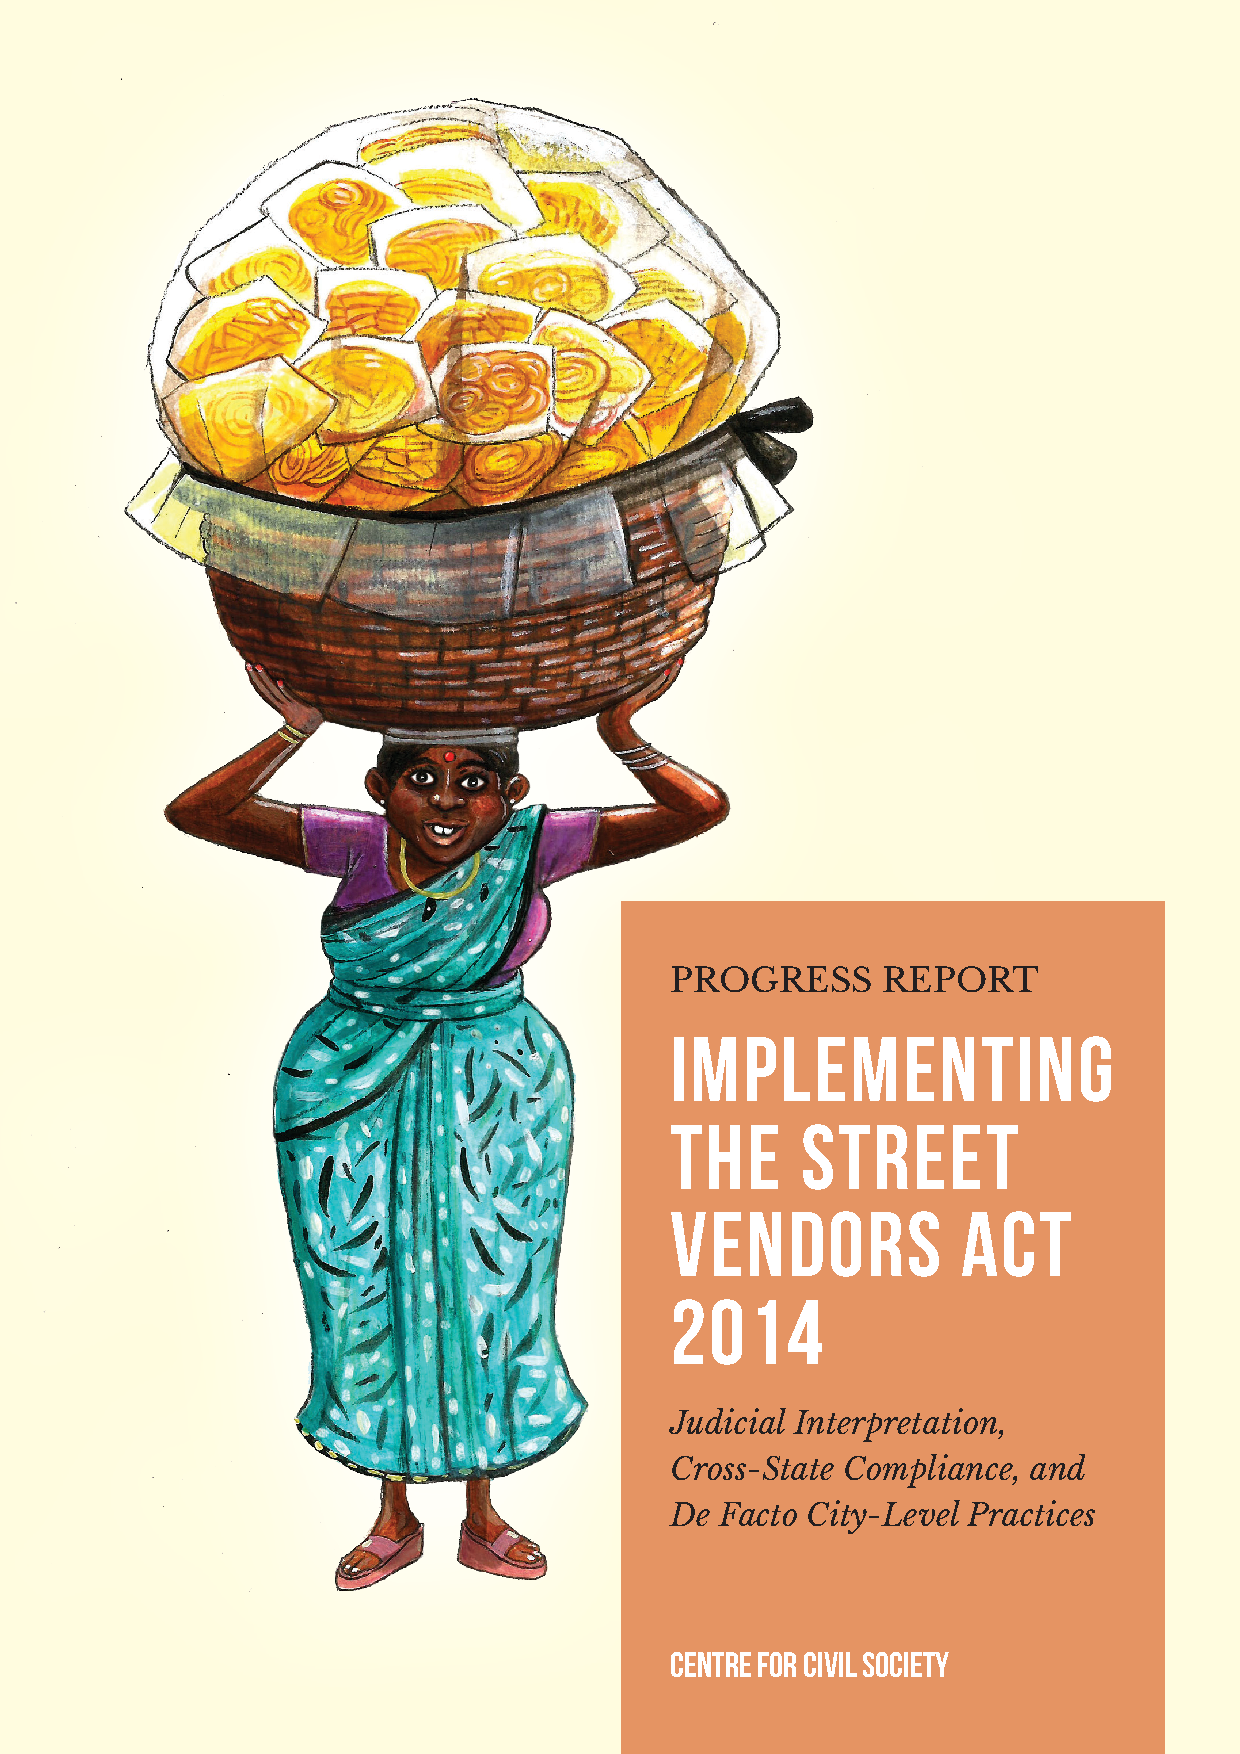
\includepdf[pages={1,2,3,4}, pagecommand={}]{Coverpage.pdf}  %attaches the pages from coverpage doc here
\pagestyle{fancy} %restarts footers from here onwards
\setcounter{page}{1} %starts counting page numbers after all the coverpages are done
\pagenumbering{arabic} %prints the new page numbers from here


%======================ACKNOWLEDGEMENTS==========================
\section*{Acknowledgements}
Centre for Civil Society (CCS) is grateful to the team at Deendayal Antyodaya Yojana-National Urban Livelihoods Mission (DAY-NULM) under Ministry of Housing and Urban Affairs (MoHUA) for providing verified state-level data at different stages of the report. We are indebted to the support and leadership of Shri Sanjay Kumar, Joint Secretary, MoHUA for providing insights and guiding our work. Transparency and open data can be powerful tools to stimulate improvements in public services and empower citizens. We hope that the ownership demonstrated by the Ministry will expedite the implementation of the Act across the country.

We would like to extend our gratitude to Shalini Sinha, India Country Representative, Women in Informal Employment: Globalizing and Organizing, for her insights and advice on our case study on Delhi.

The analysis would not have been possible without the cooperation from the survey respondents including officials of Municipal Corporation of Gurugram (MCG) and New Delhi Municipal Council (NDMC), Town Vending Committee (TVC) members (including non-government organisations, private enterprises and vendor associations) and vendors of Gurugram and Delhi.

We thank the Atlas Network for funding this year’s edition of the Progress Report on Implementing the Street Vendors Act 2014.

We are grateful to Prashant Narang for leading the legal analysis. We thank Priya Kuriyan for the illustration on the cover page, Usha Sondhi Kundu for designing the cover page and C.I. Infosolutions for proofreading the study. 

Special thanks are due to Dr Parth J Shah, President, CCS, for conceptualising the report and guiding us throughout the project. 

The research, drafting and publication of this report was carried out by the in-house team of CCS comprising Bhuvana Anand, Jayana Bedi, Alston D'Souza, Himanshu Dhingra, Pooloma Ghosh, Shruti Gupta, C. K. Pushyami, Vidushi Sabharwal, Ritika Shah and Tarini Sudhakar. 

We hope this analysis contributes to secure the rights of the street vendors, and facilitate participatory urban planning and space management.
%======================TABLE OF CONTENTS============================
\newpage
\tableofcontents

%======================LIST OF ABBREVIATIONS=========================
\newpage
\newlist{abbrv}{itemize}{1}
\setlist[abbrv,1]{label=,labelwidth=1in,align=parleft,itemsep=0.1\baselineskip,leftmargin=!}

%List of Abbreviations
\section*{Abbreviations}
\addcontentsline{toc}{section}{Abbreviations}

\begin{abbrv}[nosep]

	\item[CCS]			Centre for Civil Society
        \item[DAY-NULM]			Deendayal Antyodaya Yojana-National Urban Livelihood Mission
        \item[DCP]			Deputy Commissioner of Police
	\item[HUDA]			Haryana Urban Development Authority
	\item[MCG]			Municipal Corporation of Gurugram
	\item[MoHUA]			Ministry of Housing and Urban Affairs
	\item[NASVI]			National Association for Street Vendors India
	\item[NCR]			National Capital Region
	\item[NDMC]			New Delhi Municipal Council
	\item[NGO]			Non-Government Organisation
	\item[North DMC]			North Delhi Municipal Corporation
	\item[PWD]			Public Works Department
	\item[RTI]			Right To Information
	\item[RWA]			Residents Welfare Association
	\item[SDMC]			South Delhi Municipal Corporation
	\item[SEWA]			Self-Employed Women's Association
	\item[SSSPL]			Spick and Span Services Private Limited
	\item[SUDA-H]			State Urban Development Authority, Haryana
	\item[SUSV]			Support to Urban Street Vendors
	\item[TVC]			Town Vending Committee
	\item[ULB]			Urban Local Body
	\item[UT]			Union Territory
	\item[WIEGO]			Women in Informal Employment: Globalizing and Organizing


\end{abbrv}

%===================EXECUTIVE SUMMARY============================== %BA reviewed and edited. %BA says Please check if it fits on 2 pages, and if not let me know how many words we need to green down. 
\newpage
\section*{Executive Summary}
\addcontentsline{toc}{section}{Executive Summary}

`Informal IS normal' concluded a 2009 OECD report. Nearly 80\% of the employed population in India earns a livelihood by working in the informal economy \parencite{iloreport}. Informal employment comprises the self-employed or employees of unregistered micro-enterprises earning an honest livelihood but outside government regulation or protection. The {\href{http://mofapp.nic.in:8080/economicsurvey/pdf/032-042_Chapter_02_ENGLISH_Vol_01_2017-18.pdf}{2018 Economic Survey} estimates that 87\% of firms, contributing to 21\% of total turnover, are outside tax coverage and the social security net. Informal employment is neither illegal nor criminal, and is here to stay. 

Centre for Civil Society advances economic and property rights of such informal workers who are often at risk of abuse from authorities in absence of clear laws or bounds on state power. This report from the Centre looks at the most visible form of informal employment in urban Indian cities: street vendors.

There are several issues at the heart of the street vending debate. Assigning rights over the use of public space is one of the most contentious issues in this debate. The vendors’ right to occupation, for example, conflicts with commuters’ rights to move freely across the territory of India. The central policy problem is to manage such conflicting and competing interests of vendors, pavement users, local residents, vehicular traffic and urban space managers over the use of public space. 

The report evaluates the progress in institutionalising mechanisms to protect and regulate vending since the enactment of Street Vendors (Protection of Livelihood and Regulation of Street Vending) Act, 2014 (henceforth referred to as `the Act'). This report studies the application of new legal tools by the higher courts to resolve conflicts and evaluated the distance covered by states in implementing the Act. It has three parts: analysis of judgments; a cross-state index tracking extent and depth of implementation and case studies diving deeper into the functioning of two Town Vending Committees (TVCs) in two cities—Delhi and Gurugram. 

This year, we analysed judgments passed between January 2017 and September 2018 on disputes relating to the Act to develop a comprehensive understanding of the jurisprudence. The most contested issue continues to be the eviction of street vendors. Repeated challenges in court arise from the ambiguous legal definition of street vendors, the conflicted understanding about creating no-vending zones, and varying interpretations of the overriding effect of the Act. Far from fulfilling the intended legislative objectives, we found that the judgments passed by various High Courts failed to establish necessary checks on the actions of municipal authorities and penalised the very street vendors the Act seeks to protect.

In 2017, we developed a cross-state index and tracked the progress of individual states in implementing the Act. This year, we reassessed the status of implementation. We measured absolute and relative compliance with the Act by studying the data provided by the Ministry of Housing and Urban Affairs (MoHUA) and state governments. Five years since the enactment of the law, we found that state-level progress remains sluggish and implementation disregards several provisions of the Act. The Act states that each Urban Local Body (ULB) should have at least one TVC. Currently, there are only 2,382 TVCs for 7,263 ULBs in India. Moreover, 42\% of these TVCs do not have vendor representatives, defeating the purpose of a ‘participatory committee’. Only 4 out of 28 states and 2 Union Territories (UT) that responded to requests for data have a grievance redressal committee.

To measure the relative progress in implementing the Act, we gave each state a score based on the depth of implementation. The index captured the performance of states against the 11 steps outlined in the Act. Mizoram, Chandigarh and Rajasthan were the top three states. Two of these states previously had a State Act on vending based on the model bill provided by the central government. Though the State Acts were repealed, all orders and actions taken under them were deemed to be issued under the provisions of the Central Act and continue to be legally tenable. West Bengal and Nagaland were the worst performing states. West Bengal has 3 TVCs for 239 towns and Nagaland has 2 TVCs for 11 towns. Both states have implemented only 2 out of 11 steps. %BA says you may want to add a summary data point for Mizoram, Chandigarh and Rajasthan like for the worst states. 

Recognising the limitations inherent in self-reported data, we also studied the implementation of the Act in two cities. In Gurugram and Delhi, we assessed the disjunction between the reported and actual constitution and functioning of Town Vending Committees, an essential element of the Act. 

Gurugram is home to over 18,000 vendors. It has one TVC. While the TVC more than fulfils its representation from the local authority, government nominees, Residents Welfare Association (RWA) and market welfare associations, it falls 28\% short of the 40\% vendor representation benchmark set in the Act. The actual presence of vendor members in TVC meetings was even lower. A close reading of meeting minutes reflected that vendor views were roughshod by low numbers and by incomplete recording of their views. In the absence of a grievance redressal body to check the powers of TVC, a mechanism for vendors to obtain justice is lacking. 

In Delhi, the government has constituted 27 provisional TVCs to regulate street vendors under the Act. After some initial hiccups, the government notified Delhi Rules 2017 outlining the process to elect vendor representatives to the TVCs. The dissonance between the government’s data on the number of street vendors and civil society’s estimates is hindering true participatory governance via TVCs. For example, for the one TVC under New Delhi Municipal Council (NDMC) that we analysed, TVC members advised us that 9,000 were on the voter roll and finally only 600 were allowed to cast votes. Besides, in this particular TVC, vendors have objected to the meeting hygiene followed, such as sporadic notifications on meeting dates and times, language and comprehensiveness of meeting minutes, and the chairing of meetings by enforcement officials. In sum, the jury is out whether Delhi’s local authorities will truly hear street vendor voices and champion their protection. 

Overall, we found that despite the establishment of a comprehensive legal framework in the Act, implementation by states has been slow. We are yet to see whether the new democratic and vendor-led governance, when implemented, will lead to new ways of thinking about a place for vendors in Indian cities.

%===================Street Vendors in India: An Overview===================Ritika edited
\newpage
\section*{Street Vendors in India: An Overview}
\addcontentsline{toc}{section}{Street Vendors in India: An Overview}
Street vending or hawking constitutes a critical component of the informal economy in India, catering largely to the urban demand for affordable goods and services. An estimated 1 crore people \parencite{jhapaper} rely on street vending for their livelihoods. The ease of entry and exit, lower levels of start-up capital and flexible working hours make street vending an ideal choice for self-employment and additional income. 

Despite their contribution to the urban economy, vendors are often considered `anti-social, anti-developmental, dirty, unaesthetic and unhygienic' \parencite{wiego}. They are frequently targeted, harassed and evicted by government officials. In most cases of eviction, they reappear in connivance with municipal and police authorities. Even the Supreme Court has taken note of how vendors are a `harassed lot and are constantly victimized by the officials of the local authorities, the police, etc'. \parencite{MEHU}.

Roever (\cite*{sallypaper}) argues that economies with ambiguous laws and absence of constraints on state power encourage the low-level harassment of vendors through unofficial payment of \textit{hafta}, merchandise confiscations and periodic evictions. The lack of clarity on the rights and obligations of street vendors encourages local authorities to benefit from flourishing channels of rent seeking. 

\subsection*{What Rights Do Street Vendors Have?}
\addcontentsline{toc}{subsection}{What Rights Do Street Vendors Have?}
Street vendors operate in public spaces over which different parties claim conflicting rights. The right of a  vendor to engage in an occupation of their choice under Article 19(1)(g) may conflict with commuters’ right to move freely across the territory of India under Article 19(1)(d). 

Two kinds of rights define the ownership of a vendor over a property. The first is the `right to vend from a particular area' or rights over the immovable property hawkers operate from. The second is the `right to ownership of the movables that are used for conducting trade' \parencite{ccspaper}.

The salient policy problem, given the contrasting and often competing interests over the use of public space, is marking the precedence, extent and limits of the rights of all users. Managing conflicting claims of street vendors, pavement users, local residents, vehicular traffic and urban space managers is central to designing and implementing the regulatory framework for street vending.
\newpage
\subsection*{How Does the Street Vendors Act 2014 Apply These Rights?}
\addcontentsline{toc}{subsection}{How Does the Street Vendors Act 2014 Apply These Rights?}

\subsubsection*{Explicit Recognition of Vending as a Legitimate Livelihood}

The central government enacted the Street Vendors Act 2014, which is legally binding on all state and local governments. Prior to this, the National Policy on Urban Street Vendors 2004 was the guiding document to tackle the issues of vendors’ rights. However, the policy was only a set of guidelines and states were not legally bound to enforce it. The Act seeks to `protect the rights of urban street vendors and regulate street vending activities and matters connected therewith or incidental thereto'.

\subsubsection*{Participation of Civil Society in Spatial Regulation and Institutional Mechanisms to Protect Vendors}

\paragraph*{Protection Against Eviction:} 

The Act establishes the right to vend post-certification and payment of vending fees. It also confers upon vendors the right to movable property by creating a mechanism for them to reclaim seized goods. Moreover, Chapter 4 of the Act states that, `no street vendor shall be relocated or evicted by the local authority from the place specified in the certificate of vending unless he has been given 30 days’ notice for the same in such a manner as may be specified in the scheme'. This reduces the scope for unofficial payments, eviction and confiscation of goods by state officials. 

\paragraph*{Channel for Negotiation Between Civil Society and the State:}

The Act relegates powers to enumerate, identify and allocate vendors to zones to a TVC, allowing for decentralised governance. It redistributes powers exclusively held by municipal bodies and the police between street vendors, market associations and local residential association. To protect vendors’ rights, the Act requires at least 40\% of the TVC members to be vendors. An additional 10\% of the members must be from non-government and community-based organisations. This way the Act creates mechanisms for participatory decision making, reducing the scope for exclusionary practices such as harassment or relocation to noncommercial locations.

\paragraph*{Certify All Without Caps on the Number of Licences:} A TVC is required to conduct periodic enumeration (once every five years) of local street vendors. There is no artificial limit of the number of street vendors, creating a permitting framework instead of a licensing regime. The TVC is required to accommodate all identified vendors in the vending zones, subject to the holding capacity.\footnote{The Act defines holding capacity as `the maximum number of street vendors who can vend in any vending zone and has been determined as such by the local authority on the commendations of the Town Vending Committee'. The principles for determining holding capacity of vending zones are to be provided in the scheme for Street Vendors framed by the appropriate Government.} If the number of vendors identified exceeds the holding capacity, they are to be accommodated in an adjoining location to `avoid relocation'. The Act categorically rules out any attempt to evict or relocate vendors and declare no-vending zones, prior to the completion of the survey.

\paragraph{Ensure Grievances are Heard by an Independent Committee:} The Act mandates the state government to establish one or more independent committees, chaired by ex-judicial officers, for redressal of disputes and complaints filed by the street vendors. The Act categorically excludes any `employee of the appropriate government or the local authority' from the committee to ensure impartial decisions. In doing so, the Act recognises the need to place checks on administrative decisions and curb harassment by municipal authorities.

\subsection*{But, How Good Is the Implementation?}

In 2017, we developed an index to rank states on their progress in and fidelity to the implementation of the Act. We lodged applications under the Right to Information (RTI) Act 2005 across 30 states and UTs in India, compiled court judgements and analysed secondary sources including news stories. After collating data, we used a weighted scoring method to assess state-wise performance.

In 2018, to check progress, we systematically studied three aspects of the implementation of the Act: first, using data provided by the MoHUA and individual state governments on the status of implementation, we compiled a cross-state index measuring actual and relative progresses in implementing the Act; next, using comprehensive case law analysis of 57 court decisions,\footnote{We reviewed all judicial decisions from January 2017 to September 2018.} we studied the interpretation and precedence set by higher courts on essential elements of the Act; and finally, we evaluated the de jure and de facto functioning of TVCs in two large commercial cities—Delhi and Gurugram using semi-structured interviews with committee members. 

The report evaluates the extent of application of the new legal and governance framework to spatial conflicts and its impact on vendors. We argue that the ineffective role played by the judiciary and lackadaisical implementation by the states, makes the Act fall short of fulfilling its intended objective, that is protecting the rights of urban street vendors. 

%===================HOW HAS THE JUDICIARy INTERPRETED==================================Ritika edited
\section*{How Has the Judiciary Interpreted the Act?}
\addcontentsline{toc}{section}{How Has the Judiciary Interpreted the Act?}

The Supreme Court of India and various high courts passed 64 judgements and orders between January 2017 and September 2018 on disputes relating to the Street Vendors Act 2014. This section analyses 57 such cases to highlight the varying interpretations and discern whether these interpretations fulfil the intended legislative objectives.\footnote{Two legal repositories—Manupatra and SCC Online—were used to extract 64 unique results. Out of these 64 judgements, 57 cases were shortlisted and analysed. The rest either did not pertain to the Act or were dismissal/withdrawal orders without any discussion on merits of the case.} The section also sheds light on the most contested issues on the implementation of the Act. 

\subsection*{Summary of Issues Contested and Case Outcomes}
\addcontentsline{toc}{subsection}{Summary of Issues Contested and Case Outcomes}

\begin{itemize}
\item \textbf{Eviction is the single most contested issue:} In 47 out of 57 cases, vendors or their representatives challenged what they considered `unlawful eviction'.

\begin{itemize}
\item 	Eviction in these cases resulted mainly from: (1) the ambiguity surrounding the definition of a vendor under the law and their identification in the absence of enumeration surveys; and (2) the conflicted understanding of vending and no-vending zones, with some courts still upholding the demarcations made before the Act.

\item 	Other issues of contention relate to the representation of vendors in TVC, transparency in street vendor elections, enumeration of street vendors, permissions to change trade and implementation of the Act. 

\end{itemize}

\end{itemize}

\begin{itemize}
\item \textbf{Courts have typically decided against vendor petitions or deferred decision making in favour of maintaining the status quo} 

\begin{itemize}
\item 	Of the 57 cases, 24 cases were decided against vendors and 21 cases were deferred to the competent authority for decision making. 
\item 	Of the 24 cases where courts ruled against the vendor petitioner, 20 petitions challenged unlawful evictions or harassment. 14 out of these 20 adverse decisions were pronounced by the High Court of Delhi.
\item 	In 21 cases where courts issued deferrals, the decisions likely cemented the status quo.
\end{itemize}
\end{itemize}

\subsection*{Are Vendor Evictions Lawful?}
\addcontentsline{toc}{subsection}{Are Vendor Evictions Lawful?}

Between January 2017 and September 2018, 47 petitioners (including vendors and vendor associations) challenged what they considered unlawful eviction. Petitioners demanded protection under Section 3(3) of the Act that requires local TVCs to enumerate all existing vendors and issue identity cards before conducting any evictions. Despite the provision, vendors continue to be evicted due to various reasons especially in areas where TVCs are not functional yet. Such evictions retain historical biases against vendors. These evictions contravene the Act, which explicitly charges state machinery to take comprehensive measures to check and control the practice of forced evictions. As a result of varying judicial interpretations of the definition of a street vendor, the legal status of vendors in many places remains unclear.

\subsubsection*{Evictions Based on Exclusionary Definitions of a Street Vendor}

In cases of eviction, the first question before the Court is to determine whether the petitioner is in fact a street vendor and therefore entitled to protection under the law. A strict interpretation of the Act would suggest that until participatory governance is up and running and formal vendor enumeration is completed, all vendors are to be allowed to ply their wares. 

Two high courts—the High Court of Delhi and the High Court of Himachal Pradesh—have added new criteria to determine who is a vendor and excluded many from the ambit of legal protection under the Act. In contrast, the High Court of Kerala adopted a more progressive approach, arguing that Act extends protection to all vendors, irrespective of their current legal status.

\paragraph*{High Court of Delhi: Only Protects Vendors in Official but Outdated Lists}

The High Court of Delhi in 11 cases based its decision on the pre-2014 status of the vendor.\footnote{ Bachchu Singh v South Delhi Municipal Corporation 2017; Mahesh Kumar Yadav v North Delhi Municipal Council 2017; Raju Saha v South Delhi Municipal Corporation 2018; Sunil Kumar v Govt of NCT Delhi 2017; Girendra Pandit v South Delhi Municipal Corporation 2017; Khurshida Parveen v South Delhi Municipal Corporation 2017; Bhikki Ram and Ors v New Delhi Municipal Corporation 2017; Mohan Lal v New Delhi Municipal Council 2018; Rakesh Babu Gupta and Ors v New Delhi Municipal Council 2017; Sheetal Prasad Gupta v New Delhi Municipal Council 2017.} On the question of whether the petitioner was a licensed vendor, the Court gave primacy to the status of the petitioner as presented in three official lists: the lists of vendors prepared by the Thareja Committee in 1992, the Chopra Committee in 1996 and the NDMC in 2007. 

If the name of the petitioner was absent from any of these lists, the Court held that the petitioner was not a `regular' street vendor and, hence, not entitled to protection under Section 3(3). Even when presented with other proofs of vending identity and history, such as receipts and \textit{challans} for payments made to municipal authorities, the Court was unmoved.\footnote{These were receipts that were issued (as a part of an informal system) to the vendors in 1980s, by the municipal authorities on payment of a small sum. While the system was banned in 1998, these old receipts are still used by the vendors, to negotiate with the authorities and establish their legitimacy.}  In cases where vendors produced vending licences, the Court rejected them on the basis that the licences had expired and vendors had not taken steps to renew it. 

In \citeauthor{BhikkiRam} (\href{https://indiankanoon.org/doc/112289789/}{2017}), given the `over-crowded area,' the NDMC allowed only those vendors to vend `whose names find mention in the list of 628 eligible persons prepared by the NDMC or are licensed vendors or hawkers'. The Court chose not to interfere in the policy decision of the NDMC as long as the municipal corporation acted in a `fair, just and uniform manner without any favour of any kind'.

In three cases, where the petitioners had their names in the official lists, the Court allowed eviction but directed the municipal agencies to relocate them.\footnote{Mohan Lal v New Delhi Municipal Council 2018; Sheetal Prasad Gupta v New Delhi Municipal Council 2017; Virender v South Delhi Municipal Corporation 2017.} 

In all these instances, the Court did not heed Section 3(3) of the Act, which states that `no street vendor shall be evicted or, as the case may be, relocated till the survey... has been completed and the certificate of vending is issued to all street vendors'. Such judicial interpretation only protects a small number of vendors who have their names in official but outdated lists. Rather than penalising the tardy implementation of the Act, the Court imposes a penalty on the vendors who struggle to earn their livelihood. 

\paragraph*{High Court of Himachal Pradesh: Adds A Caveat to the Definition of Vendor:}
The High Court of Himachal Pradesh has gone a step further and added a son-of-the-soil qualification for availing protection under Section 3(3) of the Act \parencite{HariRam}. The Court stated: 

\textit{26. It is also not that every hawker has got a right of protection from ejectment/eviction, under the provisions of the Act ... There is no automatic application of the Act qua every vendor, who under misconception chooses to sit on any place or time on a public property, vending anything and everything. Persons, who come to the State, seeking employment, only on weekends or during tourist season, when tourists throng the State in large numbers, have no right of protection under the Act.}

The requirement for a vendor to be a state domicile lacks any mention in the Act, including Clauses 4 and 5 of Chapter 2 that specify the conditions for issuing a vending certificate. According to the Act, every street vendor who is above the age of 14 years and has been identified under the enumeration survey conducted by a TVC is to be issued a certificate of vending subject to certain terms and conditions. 

\paragraph*{High Court of Kerala: Set Exemplary Inclusive Parameters for Defining `Street Vendor':}

The High Court of Kerala argues that the Act extends protection to all vendors irrespective of their legal status. In 2014, it disallowed evictions and allowed the petitioner to continue vending until the procedures laid out in the Act were implemented \parencite{Thankappan}. As opposed to the narrow interpretation of the Act adopted by the High Courts of Delhi and Himachal Pradesh in 2017 to 2018, the High Court of Kerala sets a desirable example of who ought to be considered a street vendor.

\subsubsection*{Evictions Based on Pre-2014 Demarcations of No-vending Zone}

The Act prohibits municipal and local authorities from declaring no-vending zones until all vendors are listed and a TVC with vendor representation is established. Despite this, the High Court of Delhi allowed the municipal corporations to continue `regular eviction drives'. In seven cases, the Court upheld the pre-2014 demarcation by municipal bodies as an additional ground to justify eviction.\footnote{Bachchu Singh v South Delhi Municipal Corporation 2017; Arvind Gupta and Ors. v Govt. of NCT and Ors. 2017; Federation of Nehru Place Association v South Delhi Municipal Corporation and Ors. 2018; Footpath Dukandar Sangh and Ors. v State of Bihar and Ors 2017; Hari Ram v Ramesh Kumar 2017; Virender v South Delhi Municipal Corporation 2017; Vyapari Kalyan Mandal Main Pushpa v South Delhi Municipal Corporation 2017.}  Although the Court specified that such no-vending zones remain valid only until the TVCs start functioning, it allowed interim eviction. This interpretation contravenes Clause 3 of the First Schedule of the Act, which states that no-vending zone should not be declared before surveys are completed and plans formulated.

The view of the Court was challenged in \cite{VKMMP}. The petitioner argued that before 2013, the Supreme Court in Sudhir Madan v. Municipal Corporation of Delhi (2009) and Maharashtra Ekta Hawkers Union v. Municipal Corporation case (2013) directed that any new legislation, when passed, will supersede existing schemes or Acts. 

The petitioner argued that since the Act is in force, zoning demarcations should be governed by the Act and not by previous schemes or the 2009 policy. The Court however responded by noting that the Act `merely prohibits any further declaration of no-vending zones and does not nullify the existing demarcation by the municipal authorities'. On the contrary, the Court tacitly recognised that certain areas might have already been declared as no-vending zones. 

\subsubsection*{Evictions Based on Balancing `Public Interest'}

Sections 3(13) and 4(18) of the Act mandate local authorities to relocate vendors, removed from a particular area due to any public purpose, in consultation with the TVC. Judgments passed by the High Court of Delhi and the High Court of Calcutta, however, allow for evictions based on promoting public interest without any consideration for relocation.

In 2016, the High Court of Delhi allowed the civic agencies to evict vendors from no-vending zones declared prior to the enforcement of the Act to balance `public interest' (WPC 6130/2016 vide order dated 05.10.2016). In 2017, the Court argued that `Being pitched between the conflicting rights of the livelihood of the street vendors versus the life and security of the public in general, including the street vendors... we are of the opinion that the former must bow to the latter as without life and security, no question of earning a livelihood can arise' \parencite{VKMMP}.

Similarly, in 2017 \parencite{GopalS}, the High Court of Calcutta, while acknowledging that the petitioner cannot have a certificate of vending in the absence of TVCs, allowed for eviction of vendors in `public interest,' that is the construction of an underground drainage system and widening of the road. 

\subsubsection*{Evictions Based on Misinterpretation of `Overriding Effect' Clause}

Section 33 of the Act 2014 gives it an overriding effect over all other laws, whether local or state, in case of inconsistencies. This prevents harassment of street vendors on the basis of other statutes, bye-laws or executive orders. Different high courts have, however, interpreted the provision in ways that still uphold and give precedence to state and municipal laws.

\paragraph*{High Court of Kerala: Overriding Effect Only Applicable in Case of Inconsistency:}

The High Court of Kerala, in four cases, held that local permission requirements are overridden by the specific circumstances and nature of highways and that in order to vend on land abutting highways, vendors need permissions from the National Highway Authority of India or under the Highway Protection Act of the state.\footnote{Saji Joy v The Executive Engineer, Public Works Department (PWD) NH Division and Ors, 2018; Sudheesh T.S v State of Kerala and Ors, 2018; V.Prabhakaran and Ors v National Highway Authority, Kozhikode and Ors, 2018; Abbas V. and Ors v State of Kerala and Ors, 2018.} While the petitioners argued that the Act has an overriding effect, the Court observed that the effect is only applicable if there is any inconsistency. The Court held that there is nothing inconsistent between Street Vendors Act 2014, and the Control of the National Highway (Land \& Traffic) Act 2002. 

The Act, under Section 1(4), expressly excludes some areas from its purview such as railway premises, land and trains, but makes no mention of highways. The judgement of the Court, in effect, exempts highways from the coverage of the Act. 

\paragraph*{High Court of Madras: State Municipal Law Is Not Overwritten by the Act:}

The High Court of Madras held that the state municipal law—Tamil Nadu District Municipalities Act 1920—is not overwritten by the Street Vendors Act 2014 \parencite{TRamalingam}. The Court allowed eviction as the Street Vendors Act 2014 is only “to protect the livelihood rights of the street vendors and to regulate their street vending activities.” It noted that the Street Vendors Act 2014 is “regulatory in character” and the Tamil Nadu District Municipalities Act 1920, especially sections 180(A) and 182 that deal with removal of encroachment, are “mandatory”. By laying emphasis on the “mandatory” clauses of the Tamil Nadu District Municipalities Act 1920, the Court gave it precedence over and above the Street Vendors Act, 2014.




\paragraph*{High Court of Gujarat: No Protection to Vendors if State Laws are Violated:}

The High Court of Gujarat did not protect petitioners who operate `illegal and unauthorised Pucca constructions' on a public street as it violates other state laws \parencite{VakatarSG}.

\subsubsection*{Eviction Decisions Deferred to Town Vending Commitees}

The High Court of Delhi has only selectively deferred cases to the TVC. In cases where there was no ground for the dismissal of vendor petitioners, the decision was deferred to the TVC without extending any interim protection. If, however, there was a basis to dismiss the vendor petitioner (due to the legal identity of the vendor or demarcation of no-vending zones), the Court did not defer the case to the TVC and decided against the vendors. 

In \cite{VKSahu}, the petitioner-vendor contended that he had been vending at the same place for the past 21 years and was now being harassed. The area in question was not a no-vending zone, and hence the High Court of Delhi had no reason, even by its own yardstick, to deny the protection to the petitioner under Section 3(3) of the Act. Despite this, the Court deferred the decision and asked the petitioner to `approach the TVC as and when it is functional, with all the supporting documents,' without granting any interim protection.

Contrastingly, in \cite{DwarkaS6}, the Court adjudicated on two questions—whether the petitioners have been vending at a particular spot and for how many years—both being questions of fact. The Court investigated these questions, without deferring it to the TVC, and decided against the street vendors. 

When faced with similar questions, the High Courts of Madras and Kerala referred the questions of fact to the municipal agencies or the TVCs. The courts asked the municipal agency or TVC (if constituted) to consider the application filed by the petitioner-vendor within the stipulated time and decide the matter giving a reasoned order.

\subsection*{Vendors Lack Recourse to Challenge TVC Elections Voter Lists}
\addcontentsline{toc}{subsection}{Vendors Lack Recourse to Challenge TVC Elections Voter Lists}

Section 22(2)(c) of the Act mandates 40\% representation of vendors in TVC elected by the vendors themselves. However, in the absence of a legal identity of vendors in most states, `who can vote' remains a debatable question.
 
The Govt. of NCT of Delhi planned on following a two-step approach. The first step was to form TVCs elected by vendors in official lists. The second step was to task TVCs with enumerating all vendors prior to the second round of elections to form new TVCs. 

The process for election, in the first step, was challenged by vendors in \cite{RPKHU}. Petitioners argued that vendors did not have sufficient time to produce documents for verification and only 10\% of them were eligible to vote. Vendors asked the Court to issue directions to the Delhi Municipal Corporation (DMC) to: display the zone-wise voter list, allow for more time for submission of documents and allow other street vendors to raise objections against voter lists. The High Court of Delhi approved the first two demands but disallowed vendors from raising objections to voter lists as it would have led to a delay in the election process. 

A representative and well-functioning TVC is an essential feature of the Act. Disallowing vendors from raising objections against the list produced by the DMC may result in limited participation and vendor representation in TVCs. 

Apart from the varying judicial interpretations that undermine essential features of the Act, what is more intriguing is that, in a number of high courts, there are no cases related to the Act. One may understand this to be a case of either utopia or dystopia. We do not know whether this is because the high courts have not admitted any cases, or street vendors are unaware of the law, or the implementation of the law is beyond reproach. In many cases where courts have given decisions, they have allowed evictions without relocation or heed to Section 3(3) of the Act that disallows any attempt to evict until processes laid out in the Act are implemented. The role of the Court in ensuring implementation and correction of the biases cannot be understated. All vendor reforms that we see today are an effect of Supreme Court rulings through the 1990s. 

%===================HOW DO STATES FARE ON IMPLEMENTATION===========
\section*{How Far have States Progressed on Implementation?}
\addcontentsline{toc}{section}{How Far have States Progressed on Implementation?}
	Government officials—responsible for urban planning, controlling congestion, maintaining hygiene and law and order—are constantly faced with the need to `do something about street vending' \parencite{bromleypaper}. Vendors are a low priority for state governments, and governance and management of vendors is left to those at the bottom of the administrative hierarchy, including police inspectors and officials of the municipal corporation.

	Local administrators face complaints from different interest groups—residents, commuters or other vendors. Managing these conflicting demands interaction with hundreds of vendors and access to systematic information (that currently does not exist) about their identity, area of operation, or services offered. `Vendors disappear when they think they may be subject to persecution, and reappear when municipal inspectors and police have given up' \parencite{bromleypaper}. This traps vendors in complex cycles of `persecution, regulation, tolerance and promotion'.

	The Act is an attempt to systematically fill the regulatory lacuna, regularise street vendors, open channels for negotiation between stakeholders and minimise extractive opportunities. The Act identifies general principles and lays out restrictions on what can and cannot be done and leaves the application of these principles to ULBs given that regulating and managing vending requires localised solutions and consensus. But is it working?

	We identified 11 distinct steps required of state governments under the Act and gathered data to determine how far states have progressed (Table \ref{tab: SVACsteps}). We filed RTI applications in 28 states and 7 UTs asking 11 questions (one corresponding to each step) to help substantiate state progress. For example, the Act requires a state to notify the rules for implementing the Act. Correspondingly, we asked if the state government had drafted and notified the rules. Where possible, we asked for quantitative data to determine the extent of implementation. For example, on the exercise of the survey and issuance of identity cards, we asked how many vendors were identified and how many were issued identification.

%Table 1: Steps to Implement the Street Vendors Act 2014
\begin{table}[htpb]
\caption{Steps to Implement the Street Vendors Act 2014}
\label{tab: SVACsteps}
\begin{tabular}{ l  l } %Alignment of Text
\toprule
Step 1	&	State government to draft and notify the \textbf{rules} for implementing the Act\\
Step 2 	&	State government to draft and notify the \textbf{scheme} for implementing the Act\\
Step 3	&	State government to form the \textbf{Grievance Redressal Committee}\\
Step 4	&	State government to \textbf{form the TVC}\\
Step 5	&	\textbf{Election for vendor representation} in the TVC\\
Step 6	&	TVC to conduct a \textbf{survey of vendors}\\
Step 7	&	TVC to \textbf{issue identity cards} to vendors\\
Step 8	&	TVC to \textbf{earmark vending zones}\\
Step 9 	&	Local authority to draft and publish a \textbf{street vending plan}\\
Step 10	&	TVC to publish the street \textbf{vendor charter}\\
Step 11	&	Local authority to \textbf{assign office space} to the TVC\\
\bottomrule
\end{tabular}
\end{table} 

These 11 questions were also sent to the DAY-NULM. NULM sets out the strategy and operational guidelines for implementing the Act under its Support to Urban Street Vendors (SUSV) component. NULM coordinated with the state representatives multiple times and shared updated data at different stages of the report. The data was verified and updated last in January 2019.

	We received a response from 28 states and 2 UTs.\footnote{We have referred to 28 states and 2 UTs as 30 states throughout the text.} Andaman and Nicobar Island, Dadra and Nagar Haveli, Daman and Diu, Lakshadweep, and Delhi did not respond to the RTI/NULM request for data. The Act does not apply to Jammu and Kashmir. 

	In this section, we discuss our findings on the extent states have complied with the Act, four years from its onset.

\subsection*{Summary of Findings}
\addcontentsline{toc}{subsection}{Summary of Findings}

\begin{itemize}
	\item Four states \textemdash Arunachal Pradesh, Karnataka, Telangana and Nagaland\textemdash are yet to comply with step 1 on notifying the rules.
	\item 19 states have completed step 2, notification of scheme but but well after the statutory deadline of October 2014.
	\item Four states \textemdash  Assam, Madhya Pradesh, Punjab and Uttarakhand\textemdash have implemented step 3, the formation of the Grievance Redressal Committees.
	\item Of the 7,263 towns from 30 states, 33\% have complied with step 4, formation of TVC.
	\item Of the 2,382 TVCs formed, 58\% have complied with step 5, vendor representation in the TVCs.
	\item Of the TVCs formed, 98\% have completed step 6, vendor enumeration.
	\item Of the TVCs formed, 50\% have issued identity cards to 75\% of the identified vendors.
	\item Of the TVCs formed, 20\% have complied with step 8 and have a street vending plan based on which vending zones are to be earmarked (step 9). 
	\item Of the TVCs formed, 31\% have complied with step 10 and published a street vendor charter.
\end{itemize}

\subsection*{26 States Have Drafted and Notified the Rules}
\addcontentsline{toc}{subsection}{26 States Have Drafted and Notified the Rules}
	The Act mandates, `The appropriate government shall, within one year from the date of commencement of this Act, by notification, make rules for carrying out the provisions of this Act'. The rules lay down the guidelines for implementation such as the minimum age of the vendor, processes for forming TVC, electing vendors representatives to the TVC, filing appeals in cases of disputes and for drafting and notifying the scheme.

	Four states—Arunachal Pradesh, Karnataka, Telangana and Nagaland—are yet to notify rules.

	Arunachal Pradesh repealed the Arunachal Pradesh Street Vendors Act 2011, in March 2018 and came under the purview of the Central Act with effect from May 2018.\footnote{The Arunachal Pradesh Street Vendors (Protection of Livelihood and Regulation of Street Vending)(Repeal) Bill,2018} The repeal of the state Act and the adoption of Central Act partially explain the delay in notifying the rules. The state, however, already has TVCs in 45\% of its town. In the absence of the rules, the legal tenability of the committees is in question.

\subsection*{19 States Have Drafted and Notified the Scheme}
\addcontentsline{toc}{subsection}{19 States Have Drafted and Notified the Scheme}
	Section 38 of the Act requires state governments to frame and notify a scheme within 6 months from May 2014, with due consultation from the local authority and the TVC. 11 states—Arunachal Pradesh, Gujarat, Haryana, Karnataka, Kerala, Madhya Pradesh, Manipur, Nagaland, Puducherry, Sikkim and West Bengal—are yet to notify the scheme.

	The scheme is to provide the TVC with guidelines to conduct the survey of vendors and defines the manner and process for issuing identity cards and its content. TVCs have to follow the processes specified in the scheme to issue licences, mark vending zones, evict or relocate vendors and determine vending fees. A thoughtful and detailed scheme provides vendors with legal protection against informal governance practices—hafta collection, seizure of goods and sudden eviction.

\subsection*{Four States Have Formed Grievance Redressal Committees}
\addcontentsline{toc}{subsection}{Four States Have Formed Grievance Redressal Committees}
	Section 20 of the Act requires the formation of one or more Grievance Redressal Committees `consisting of a chairperson who has been a civil judge or a judicial magistrate and two other professionals'. Only four states—Assam, Madhya Pradesh, Uttarakhand and Punjab—have formed Grievance Redressal Committees.

\subsection*{Of the 7,263 Towns from 30 States, 33\% Have Formed TVCs}
\addcontentsline{toc}{subsection}{Of the 7,263 Towns from 30 States, 33\% Have Formed TVCs}
	Section 22(1) of the Act gives the power to the state government to decide the number of TVCs that may be constituted under each local authority. We assume that ‘local authority’ refers to a ULB.

	14 states—Andhra Pradesh, Bihar, Chandigarh, Goa, Gujarat, Haryana, Kerala, Meghalaya, Mizoram, Puducherry, Punjab, Rajasthan, Telangana and Tripura—have formed TVCs in all their towns. Of these, Karnataka and Telangana do not have rules in places, and therefore the process with which the TVCs have been formed remains questionable.

	A TVC is responsible for conducting vendor enumeration and issuing identity cards and certificates of vending. This is the first step towards protecting and regulating vendors. Each year of delay in setting up TVCs imposes costs on vendors in the form of bribes to government officials, penalties during evictions, loss of livelihood in case of eviction and loss of goods during seizure. A study in 8 markets in Delhi estimated this loss at Rs 140 crore for 8,150 vendors annually \parencite{ratanpaper}.

\subsection*{Of the 2,382 TVCs Formed, 58\% Claim to Have Vendor Representation}
\addcontentsline{toc}{subsection}{Of the 2,382 TVCs Formed, 58\% Claim to Have Vendor Representation}
	
	The Act mandates at least 40\% vendor representation in any TVC. Further, 1,391, accounting for 58\% of TVCs, have representation from vendors.

	Per the Act, the state is to define the manner and process of electing vendors in the rules. A close look at the rules shows that not all states have chosen `election' to appoint vendor representative. Andhra Pradesh rules, for example, allow for vendors to apply for appointment and if the applications are higher than required, the local authority selects by lottery. Himachal Pradesh, Haryana and Karnataka, have provisional TVCs, with nominated vendors till such time that the survey is completed. Punjab has elected vendors to the TVC but by `show of hands in the presence of the Chairperson of the Town Vending Committee'.
	
\subsection*{98\% of TVCs Formed Have Enumerated Vendors}
\addcontentsline{toc}{subsection}{98\% of TVCs Formed Have Enumerated Vendors}
	
	Section 3 of the Act mandates the TVC to enumerate vendors as prescribed in the state scheme. 98\% of the 2,382 TVCs have completed vendor enumeration.

	Eight states—Arunachal Pradesh, Gujarat, Haryana, Karnataka, Kerala, Madhya Pradesh, Manipur, and Puducherry—however, have enumerated vendors without a scheme. In the absence of formal guidelines, the TVCs are not bound to issue public notices before the enumeration process. Poor information may result in vendor exclusion and force them to operate illegally.

\subsection*{50\% of TVCs Formed Have Issued Identity Cards to 75\% of Identified Vendors}
\addcontentsline{toc}{subsection}{50\% of TVCs Formed Have Issued Identity Cards to 75\% of Identified Vendors}

	A TVC, under Section 6 of the Act, is required to issue identity cards to every street vendor identified in the enumeration process. Further, 50\% of all TVCs formed have issued identification to 75\% of enumerated vendors. Five states—Arunachal Pradesh, Gujarat, Kerala, Manipur and Puducherry—have distributed identity cards without a scheme.

	In the absence clear guidelines for enumeration, governing bodies may apply numerical limits on licences encouraging extractive opportunities and limiting due process.

\subsection*{20\% of the TVCs Have A Published Street Vending Plan}
\addcontentsline{toc}{subsection}{20\% of the TVCs Have A Published Street Vending Plan}
	The local authority, under Section 21, is required to frame a plan of vending based on recommendations from the TVC. The plan covers elements such as criteria for earmarking no-vending zones, restricted zones, vending zones, and natural markets.

	Selected TVCs in Madhya Pradesh, Maharashtra, Meghalaya, Nagaland and Punjab have demarcated vending zones without a vending plan. The Act upholds certain principles for demarcating the vending zone. For example, a plan must `ensure that the provision of space or area for street vending is reasonable and consistent with existing natural markets'. Without a vending plan, the basis of demarcation is not clear and there is no way to verify whether if it upholds the principles specified in the Act.

\subsection*{31\% of TVCs Have Published the Street Vendor Charter}
\addcontentsline{toc}{subsection}{31\% of TVCs Have Published the Street Vendor Charter}
	Section 26 of the Act mandates the TVC to publish a street vendor charter specifying the time of renewal of vendor identity cards and for maintaining updated records of registered street vendors.

	Further, 31\% of total TVCs formed have published the charter. These belong to seven states—Bihar, Madhya Pradesh, Maharashtra, Odisha, Puducherry, Rajasthan and Tamil Nadu.

\subsection*{Six States Have Assigned Office Space to TVCs}
\addcontentsline{toc}{subsection}{Six States Have Assigned Office Space to TVCs}
	According to Section 25 of the Act, `The local authority shall provide the Town Vending Committee with appropriate office space and such employees as may be prescribed'. Six states have assigned office space to TVCs (Table \ref{tab: OfficeSpace}).


%Table 2: States Where TVCs Have Assigned Office Space
\begin{table}[htpb]
\caption{States Where TVCs Have Assigned Office Space}
\label{tab: OfficeSpace}
\begin{tabular}{ l  r r r } %Alignment of Text
\toprule
\multicolumn{1}{p{0.5em}}{States} & \multicolumn{1}{>{\raggedright\arraybackslash}p{6.7em}}{Assigned Office Space to TVCs} & \multicolumn{1}{>{\raggedright\arraybackslash}p{10em}}{Number of TVCs with Assigned Office Space} & \multicolumn{1}{>{\raggedright\arraybackslash}p{11em}}{Percentage of TVCs with Assigned Office Space}\\
\midrule
Chandigarh & 1 & 1 & 100\\
Madhya Pradesh & 364 & 58 & 16\\
Manipur & 28 & 6 & 21\\
Puducherry & 5 & 5 & 100\\
Punjab & 165 & 163 & 99\\
Rajasthan & 189 & 189 & 100\\
\bottomrule
\end{tabular}
\end{table}

%===================WHICH STATES HAVE DONE BETTER===================
\section*{Which States Have Done Better than the Others?}
\addcontentsline{toc}{section}{Which States Have Done Better Than The Others?}
	In this section, we score each state based on the extent to which they have implemented a step. The index captures depth of state performance on all 11 steps (Table \ref{tab: SVACsteps}).

	The 2018 index has been modified in two ways from the previous edition. First, we have replaced some steps such as `town vending committee first meeting' and `summary of scheme in two local newspapers' with new steps including the issuance of identity cards, development of street vending plan, and demarcation of vending zones. Second, instead of relying only on an ordinal scale, we have considered the depth of implementation wherever possible. For example, we have calculated the proportion of TVCs that have enumerated vendors, issued identity cards or published the plan. For other steps such as the notification of rules and schemes, we have assigned an ordinal value of 1 if it is complete and 0, if not. These values are then multiplied by the weight for the step (Appendix \ref{appendix: formula}). The state score is a sum of these mixed values.

	Despite the adoption of new ways to refine and strengthen the methodology, the index should be read with certain caveats. The data is self-reported by states. Moreover, in the absence of sufficient municipality information, it is at best suggestive of the compliance and implementation at the local level. The Act creates scope for local participation, and a close look at the plans, schemes, rules, orders, circulars, and meeting minutes is necessary to comment on whether implementation is promoting or suppressing justice. Finally, it does not capture state-specific idiosyncrasies that may influence state performance. For example, Mizoram, with the second highest score of 75, was one of the five states to have an Act on vending—the Mizoram Street Vendor (Protection of Livelihood and Regulation of Street Vending) Act 2011—based on the model bill provided by the central government. The state Act was repealed in 2017. All orders and actions under the 2011 Act, however, are deemed to be issued under the provisions of the Central Act and, thus, are legally tenable. This gives Mizoram an advantage as some TVCs were already in place, and they remain valid even after the introduction of the Act.

	Despite the shortcomings, the index gives a bird’s eye view of implementation and offers a starting point for further enquiry. It induces federal competition between states and pushes them to outperform each other, especially if performance is tied to monetary grants.

	\textit{Tables \ref{tab: Ranking} and \ref{tab: Index} give the rankings and step-level information to highlight areas of improvement for each state.}

%Table 3: Compliance of States with the Act: Ranking Based on the Depth of Implementation of Each Step

\newpage
\footnotesize
\begin{longtable}[l]{>{\raggedright}p{4cm}>{\raggedright\arraybackslash}p{10cm}}
\caption{Compliance of States with the Act: Ranking Based on the Depth of Implementation of Each Step}
\label{tab: Ranking}\\
	\toprule
	States & Insights \\
	\midrule
	\endfirsthead
	States & Insights \\
	\midrule
	\endhead
	\bottomrule
	\endfoot
	\endlastfoot
	\multicolumn{2}{l}{States with Best Compliance (Index Score Equal to or Above 70)}\\
	\midrule
\cellcolor{SVACgreen1}\bf{Tamil Nadu}
\newline
Score: 76
\newline
Steps: 8/11
&
\cellcolor{SVACgreen2}482 TVCs have enumerated vendors in 664 town, out of the total 721 towns in the state.  It is possible that one TVC is administering enumeration of the vendors in more than one town. 
 \\
 
%\cellcolor{SVACgreen1} & \cellcolor{SVACgreen2}
\cellcolor{SVACgreen1}\bf{Mizoram}
\newline
\bf{Score: 75}
\newline
\bf{Steps: 8/11}
&
\cellcolor{SVACgreen2}All six towns have a TVC with vendor representatives. The TVCs, however, do not have an assigned office space and have not published the charter. There are no Grievance Redressal Committees.
\\
\cellcolor{SVACgreen1}\bf{Chandigarh}
\newline
\bf{Score: 75}
\newline
\bf{Steps: 8/11}
&
\cellcolor{SVACgreen2}There is one TVC with elected vendor representatives. It has identified 9,353 vendors but has not issued identity cards or published the charter. There are no Grievance Redressal Committees.
\\
\cellcolor{SVACgreen1}\bf{Rajasthan}
\newline
\bf{Score: 70}
\newline
\bf{Steps: 10/11}
&
\cellcolor{SVACgreen2}Per the Act, the vending zones should be earmarked following the guidelines laid down in the vending plan. While 4\% of the towns have published the plan, 67\% of TVCs have already earmarked vending zones.
\\
\midrule
\multicolumn{2}{l}{States with Good Compliance (Index score Between 50 to 69)}\\
\midrule
\cellcolor{SVACgreen3}\bf{Jharkhand}
\newline
\bf{Score: 69}
\newline
\bf{Steps: 8/11}
&
\cellcolor{SVACgreen2}While 48\% of the TVCs have a published vending plan, 77\% of the TVCs have earmarked vending zones.
\\
\cellcolor{SVACgreen3}\bf{Himachal Pradesh}
\newline
\bf{Score: 68}
\newline
\bf{Steps: 8/11}
&
\cellcolor{SVACgreen2}93\% of the towns have formed a TVC. Per the rules notified in December 2016, the TVCs are provisional and will be replaced once survey and election of vendors are complete. Until then, the vendor representatives are nominated.

Although only 39 towns have TVCs, vendor enumeration is complete in 41 towns. It is possible that one TVC is administering enumeration in more than one town.
\\
\cellcolor{SVACgreen3}\bf{Uttar Pradesh}
\newline
\bf{Score: 67}
\newline
\bf{Steps: 8/11}
&
\cellcolor{SVACgreen2}30 out of 130 towns have formed a TVC with vendor representation. The representation is not through election, but selection of applicants from vendor associations. The 30 TVCs have enumerated vendors and issued identity cards. 13 TVCs have earmarked vending zones even without a plan in place.
\\
\cellcolor{SVACgreen3}\bf{Andhra Pradesh}
\newline
\bf{Score: 66}
\newline
\bf{Steps: 8/11}
&
\cellcolor{SVACgreen2}In Andhra Pradesh 1 town has published the plan but 40 TVCs have earmarked vending zones. It is not clear whether one plan is being used to earmark vending zones in all 40. If not, then how have TVCs earmarked no-vending, restricted vending and vending zones? What are the spatial planning norms used?
\\
\cellcolor{SVACgreen3}\bf{Puducherry}
\newline
\bf{Score: 66}
\newline
\bf{Steps: 8/11}
&
\cellcolor{SVACgreen2}Puducherry has complied fully with all steps except three: notification of scheme, constitution of a Grievance Redressal Committee, and appointment of vendor representatives in the TVCs. Enumeration, registration and demarcation of vending zones without vendor representatives in the TVC defeat the purpose of a participatory committee.
\\
\cellcolor{SVACgreen3}\bf{Punjab}
\newline
\bf{Score: 65}
\newline
\bf{Steps: 9/11}
&
\cellcolor{SVACgreen2}Punjab is one of the four states that have formed the Grievance Redressal Committee. The Act mandates the state to define the process of election for representing vendors in the TVC. Punjab has used \textit{show of hands} as the way to elect vendors. On the basis of  this, all 165 towns have vendor representation in the TVCs. In the absence of a vending plan, vending zones have been earmarked in three towns.
\\
\cellcolor{SVACgreen3}\bf{Odisha}
\newline
\bf{Score: 61}
\newline
\bf{Steps: 9/11}
&
\cellcolor{SVACgreen2}Odisha has implemented 9 out of 11 steps: all 105 towns have formed a TVC with elected vendor representation; 79\% of the TVCs have enumerated vendors; 14 TVCs have issued identity cards and 5\% of the towns have published a plan and earmarked vending zones.
\\
\cellcolor{SVACgreen3}\bf{Goa}
\newline
\bf{Score: 60}
\newline
\bf{Steps: 8/11}
&
\cellcolor{SVACgreen2}Goa has formed TVCs in all 14 towns with street vendor representatives. Only two TVCs have issued ID cards and four have earmarked vending zones. There are no Grievance Redressal Committees.
\\
\cellcolor{SVACgreen3}\bf{Gujarat}
\newline
\bf{Score: 53}
\newline
\bf{Steps: 7/11}
&
\cellcolor{SVACgreen2}Gujarat has notified the rules, not the scheme. A scheme is to specify the manner of conducting the survey and the form and manner of issuing ID cards. In the absence of a scheme, 168 out of 169 TVCs have already completed the enumeration exercise and issued identification to more than 75\% vendors.
\\
\cellcolor{SVACgreen3}\bf{Telangana}
\newline
\bf{Score: 50}
\newline
\bf{Steps: 5/11}
&
\cellcolor{SVACgreen2}Due to the dissolution of the state government in early 2017, there has been a delay in notifying the rules. However, the state has published the scheme.

74 towns in the state have formed 103 TVCs with elected vendors.
\\
\midrule
\multicolumn{2}{l}{States with Moderate Compliance (Index Score Between 30 to 49)}\\
\midrule
\cellcolor{SVACyellow1}\bf{Bihar}
\newline
\bf{Score: 47}
\newline
\bf{Steps: 8/11}
&
\cellcolor{SVACyellow2}All 144 towns have formed a TVC without vendor representation. Only 3 towns have published the plan but 46 TVCs have already earmarked vending zones.
\\
\cellcolor{SVACyellow1}\bf{Uttarakhand}
\newline
\bf{Score: 47}
\newline
\bf{Steps: 6/11}
&
\cellcolor{SVACyellow2}In Uttarakhand, 40 out of 93 towns have a TVC. Vendor enumeration is complete in 55 towns. 10 TVCs have issued identity cards to more than 75\% of vendors. However, none of the TVCs have vendor representatives so far.
\\
\cellcolor{SVACyellow1}\bf{Madhya Pradesh}
\newline
\bf{Score: 46}
\newline
\bf{Steps: 8/11}
&
\cellcolor{SVACyellow2}Madhya Pradesh has implemented 8 out of 11 steps in less than a third of the towns.
\\
\cellcolor{SVACyellow1}\bf{Haryana}
\newline
\bf{Score: 45}
\newline
\bf{Steps: 5/11}
&
\cellcolor{SVACyellow2}In Haryana, there are 80 TVCs for 80 towns. None of the TVCs have vendor representatives. The state has not notified the scheme but has completed enumeration in all towns; 58 towns have a plan but 72 have earmarked vending zones.
\\
\cellcolor{SVACyellow1}\bf{Chhattisgarh}
\newline
\bf{Score: 45}
\newline
\bf{Steps: 5/11}
&
\cellcolor{SVACyellow2}64 out of 169 towns in Chhattisgarh have a TVC but without vendor representation. All 64 TVCs have completed the survey. Also, 35 TVCs have issued ID cards to more than 75\% of identified vendors.
\\
\cellcolor{SVACyellow1}\bf{Meghalaya}
\newline
\bf{Score: 43}
\newline
\bf{Steps: 6/11}
&
\cellcolor{SVACyellow2}In Meghalaya, there are seven TVCs but without vendor representation. One town has marked vending zones but without a plan.
\\
\cellcolor{SVACyellow1}\bf{Tripura}
\newline
\bf{Score: 40}
\newline
\bf{Steps: 4/11}
&
\cellcolor{SVACyellow2}Tripura has formed TVCs in all 20 towns but only 25\% of the TVCs have enumerated vendors.
\\
\cellcolor{SVACyellow1}\bf{Assam}
\newline
\bf{Score: 39}
\newline
\bf{Steps: 5/11}
&
\cellcolor{SVACyellow2}Assam is one of the four states that have formed Grievance Redressal Committees.
\\
\cellcolor{SVACyellow1}\bf{Kerala}
\newline
\bf{Score: 37}
\newline
\bf{Steps: 4/11}
&
\cellcolor{SVACyellow2}Kerala has a TVC in all its towns but without vendor representation. Vendor enumeration is complete in all TVCs and 35\% of these TVCs have issued identity cards, without a scheme in place.
\\
\cellcolor{SVACyellow1}\bf{Arunachal Pradesh}
\newline
\bf{Score: 34}
\newline
\bf{Steps: 6/11}
&
\cellcolor{SVACyellow2}Arunachal Pradesh is one of the four states without rules in place. The delay in the implementation may be attributed to the time taken to repeal the State Act---Arunachal Pradesh Street Vendors Act 2011. Even though the repeal saved all orders and actions taken under the 2011 Act, the state still fares low. It is possible that not much progress was made under the previous Act.

\\
\cellcolor{SVACyellow1}\bf{Maharashtra}
\newline
\bf{Score: 32}
\newline
\bf{Steps: 7/11}
&
\cellcolor{SVACyellow2}97 out of 3,799 towns have formed a TVC.
\\
\midrule
\multicolumn{2}{l}{States with Poor Compliance (Index Score Between 10 to 29)}\\
\midrule
\cellcolor{SVACred1}\bf{Manipur}
\newline
\bf{Score: 29}
\newline
\bf{Steps: 7/11}
&
\cellcolor{SVACred2}Manipur has enumerated vendors, issued identity cards, published a plan and earmarked vending zones but in the absence of a scheme.
\\
\cellcolor{SVACred1}\bf{Karnataka}
\newline
\bf{Score: 23}
\newline
\bf{Steps: 4/11}
&
\cellcolor{SVACred2}Karnataka has formed 265 TVCs in 237 towns. The TVCs have enumerated vendors as well. However, the state has not yet notified the rules or the scheme, raising questions on the tenability of the progress.
\\
\cellcolor{SVACred1}\bf{Sikkim}
\newline
\bf{Score: 21}
\newline
\bf{Steps: 2/11}
&
\cellcolor{SVACred2}Sikkim has not yet published the scheme.
\\
\cellcolor{SVACred1}\bf{West Bengal}
\newline
\bf{Score: 13}
\newline
\bf{Steps: 2/11}
&
\cellcolor{SVACred2}West Bengal has notified the rules and formed TVCs in 3 out of 239 towns, accounting for 1\%, the lowest among all states.
\\ 
\midrule
\multicolumn{2}{l}{States with Very Poor Compliance (Index Score Equal to or Less than 9)}\\
\midrule
\cellcolor{SVACred3}\bf{Nagaland}
\newline
\bf{Score: 9}
\newline
\bf{Steps: 2/11}
&
\cellcolor{SVACred2}Nagaland has not notified rules and scheme. It has formed TVCs in 2 out of 11 towns and has earmarked vending zones in the two areas.\\
\bottomrule
	\end{longtable}
\normalsize


%Table X: Step-Wise Data on Implementation for 30 states, as of October 31 2019

%BA says revise date convention everywhere to dd Month YYYY please. BA says have not been able to read table
           \scriptsize
             \begin{landscape}
  \rowcolors{2}{gray!25}{white}
  \centering
            \begin{longtable}{p{2cm}p{0.5cm}p{0.5cm}>{\raggedleft}p{0.5cm}>{\raggedleft}p{0.5cm}>{\raggedleft}p{0.5cm}>{\raggedleft}p{0.5cm}>{\raggedleft}p{0.5cm}>{\raggedleft}p{0.5cm}>{\raggedleft}p{0.5cm}>{\raggedleft}p{0.5cm}>{\raggedleft}p{1.0cm}>{\raggedleft}p{0.5cm}>{\raggedleft}p{0.5cm}>{\raggedleft}p{0.5cm}>{\raggedleft}p{0.5cm}>{\raggedleft}p{0.5cm}>{\raggedleft}p{0.5cm}>{\raggedleft}p{0.5cm}>{\raggedleft}p{0.5cm}>{\raggedleft}p{0.5cm}>{\raggedleft\arraybackslash}p{0.5cm}}
            \caption{Step-Wise Data on Implementation for 30 states, as of 31 October 2018}
            \label{tab: Index}\\
States &
\rotatebox{90}{Rules} &
\rotatebox{90}{Scheme} &
\rotatebox{90}{Towns} &
\rotatebox{90}{Total TVCs} &
\rotatebox{90}{\thead{Total TVCs/ \\ Total towns (\%)}} &
\rotatebox{90}{\thead{Have vendor \\ representatives}} &
\rotatebox{90}{\thead{\% of TVCs with \\ vendor representatives}} &
\rotatebox{90}{Completed enumeration} &
 \rotatebox{90}{\thead{\% of TVCs that \\ completed enumeration}} &
 \rotatebox{90}{\thead{Issued IDs to \textgreater 75\% \\ vendors}} &
 \rotatebox{90}{\thead{\% of TVCs that \\ issued ID \textgreater 75\% of \\ identified vendors}} &
 \rotatebox{90}{Published plan} &
 \rotatebox{90}{\thead{\% of TVCs with \\ published plan}} &
 \rotatebox{90}{Vending zones} &
 \rotatebox{90}{\thead{\% of TVCs that marked \\ vending zones}} &
 \rotatebox{90}{Published charter} &
 \rotatebox{90}{\thead{\% of TVCs that \\ published charter}} &
 \rotatebox{90}{Assigned office space} &
 \rotatebox{90}{\thead{\% of TVCs that have \\ assigned office space}} &
 \rotatebox{90}{\# of GRCs in the state} &
 \rotatebox{90}{\% of towns with GRC} \\

AP & Y & Y & 110 & 110 & 100 & 110 & 100 & 110 & 100 & 85 & 77 & 1 & 1 & 50 & 45 & 0 & 0 & 0 & 0 & 0 & 0 \\
AR & N & N & 33 & 15 & 45 & 10 & 67 & 14 & 93 & 14 & 93 & 8 & 53 & 4 & 27 & 0 & 0 & 0 & 0 & 0 & 0 \\
AS & Y & Y & 110 & 24 & 22 & 0 & 0 & 24 & 100 & 0 & 0 & 0 & 0 & 0 & 0 & 0 & 0 & 0 & 0 & 4 & 4 \\
BR & Y & Y & 144 & 144 & 100 & 0 & 0 & 46 & 32 & 42 & 29 & 3 & 2 & 46 & 32 & 42 & 29 & 0 & 0 & 0 & 0 \\
CH & Y & Y & 1 & 1 & 100 & 1 & 100 & 1 & 100 & 0 & 0 & 1 & 100 & 1 & 100 & 0 & 0 & 1 & 100 & 0 & 0 \\
CG & Y & Y & 169 & 64 & 38 & 0 & 0 & 64 & 100 & 35 & 55 & 0 & 0 & 0 & 0 & 0 & 0 & 0 & 0 & 0 & 0 \\
GA & Y & Y & 14 & 14 & 100 & 14 & 100 & 11 & 79 & 2 & 14 & 4 & 29 & 4 & 29 & 0 & 0 & 0 & 0 & 0 & 0 \\
GJ & Y & N & 169 & 169 & 100 & 12 & 7 & 168 & 99 & 168 & 99 & 131 & 78 & 131 & 78 & 0 & 0 & 0 & 0 & 0 & 0 \\
HR & Y & N & 80 & 80 & 100 & 0 & 0 & 80 & 100 & 0 & 0 & 58 & 73 & 72 & 90 & 0 & 0 & 0 & 0 & 0 & 0 \\
HP & Y & Y & 54 & 39 & 72 & 39 & 100 & 40 & 103 & 9 & 23 & 31 & 79 & 25 & 64 & 0 & 0 & 0 & 0 & 0 & 0 \\
JH & Y & Y & 48 & 44 & 92 & 44 & 100 & 44 & 100 & 22 & 50 & 21 & 48 & 34 & 77 & 0 & 0 & 0 & 0 & 0 & 0 \\
KA & N & N & 271 & 265 & 98 & 0 & 0 & 265 & 100 & 0 & 0 & 4 & 2 & 4 & 2 & 0 & 0 & 0 & 0 & 0 & 0 \\
KL & Y & N & 93 & 93 & 100 & 0 & 0 & 93 & 100 & 33 & 35 & 0 & 0 & 0 & 0 & 0 & 0 & 0 & 0 & 0 & 0 \\
MP & Y & N & 364 & 58 & 16 & 58 & 100 & 58 & 100 & 0 & 0 & 0 & 0 & 58 & 100 & 4 & 7 & 58 & 100 & 3 & 1 \\
MH & Y & Y & 3799 & 97 & 3 & 24 & 25 & 17 & 18 & 0 & 0 & 0 & 0 & 8 & 8 & 7 & 7 & 0 & 0 & 0 & 0 \\
MN & Y & N & 28 & 6 & 21 & 0 & 0 & 2 & 33 & 1 & 17 & 2 & 33 & 2 & 33 & 0 & 0 & 6 & 100 & 0 & 0 \\
ML & Y & Y & 7 & 7 & 100 & 0 & 0 & 3 & 43 & 1 & 14 & 0 & 0 & 1 & 14 & 0 & 0 & 0 & 0 & 0 & 0 \\
MZ & Y & Y & 6 & 6 & 100 & 6 & 100 & 6 & 100 & 5 & 83 & 5 & 83 & 5 & 83 & 0 & 0 & 0 & 0 & 0 & 0 \\
NL & N & N & 11 & 2 & 18 & 0 & 0 & 0 & 0 & 0 & 0 & 0 & 0 & 2 & 100 & 0 & 0 & 0 & 0 & 0 & 0 \\
OD & Y & Y & 112 & 104 & 93 & 104 & 100 & 111 & 107 & 21 & 20 & 5 & 5 & 5 & 5 & 15 & 14 & 0 & 0 & 0 & 0 \\
PY & Y & N & 5 & 5 & 100 & 0 & 0 & 5 & 100 & 5 & 100 & 5 & 100 & 5 & 100 & 5 & 100 & 5 & 100 & 0 & 0 \\
PB & Y & Y & 165 & 165 & 100 & 165 & 100 & 163 & 99 & 61 & 37 & 0 & 0 & 3 & 2 & 0 & 0 & 163 & 99 & 13 & 8 \\
RJ & Y & Y & 189 & 189 & 100 & 189 & 100 & 189 & 100 & 85 & 45 & 7 & 4 & 126 & 67 & 1 & 1 & 189 & 100 & 0 & 0 \\
SK & Y & N & 4 & 3 & 75 & 0 & 0 & 0 & 0 & 0 & 0 & 0 & 0 & 0 & 0 & 0 & 0 & 0 & 0 & 0 & 0 \\
TN & Y & Y & 721 & 482 & 67 & 482 & 100 & 664 & 138 & 482 & 100 & 164 & 34 & 0 & 0 & 664 & 138 & 0 & 0 & 0 & 0 \\
TS & N & Y & 74 & 103 & 139 & 103 & 100 & 66 & 64 & 72 & 70 & 0 & 0 & 0 & 0 & 0 & 0 & 0 & 0 & 0 & 0 \\
TR & Y & Y & 20 & 20 & 100 & 0 & 0 & 5 & 25 & 0 & 0 & 0 & 0 & 0 & 0 & 0 & 0 & 0 & 0 & 0 & 0 \\
UP & Y & Y & 130 & 30 & 23 & 30 & 100 & 30 & 100 & 30 & 100 & 16 & 53 & 29 & 97 & 0 & 0 & 0 & 0 & 0 & 0 \\
UK & Y & Y & 93 & 40 & 43 & 0 & 0 & 55 & 138 & 10 & 25 & 0 & 0 & 0 & 0 & 0 & 0 & 0 & 0 & 1 & 1 \\
WB & Y & N & 239 & 3 & 1 & 0 & 0 & 0 & 0 & 0 & 0 & 0 & 0 & 0 & 0 & 0 & 0 & 0 & 0 & 0 & 0 \\
\midrule
Sum Total / \% & 0 & 0 & 7263 & 2382 & 33 & 1391 & 58 & 2334 & 98 & 1183 & 50 & 466 & 20 & 615 & 26 & 738 & 31 & 422 & 18 & 21 & 13 \\
No. of States that Initiated Work & 24 & 0 & & 30 & & 16 & & 27 &  & 20 &  & 17 &  & 21 &  & 7 &  & 6 &  & 4 & 4 \\

\end{longtable}
\end{landscape}
\normalsize
%===================LESSONS FROM THE FIELD==========================
\section*{Closer to the Field: Challenges in Implementation}
\addcontentsline{toc}{section}{Closer to the Field: Challenges in Implementation}


Measuring compliance, based on quantitative indicators, only serves as a starting point of enquiry into whether and how the new Act redefines the regulatory environment for street vendors. Numbers may or may not capture the disjunction between ideas, institutions and practices that local administrators ultimately adopt.

Keeping this disjunction in mind, we use a case study approach to study a small but a critical unit of governance, the TVC.

The provision of a TVC, the local participatory body comprising representatives from local authorities, vendors, market and residential associations, creates a platform for stakeholders with competing and conflicting interests to contribute to critical decisions. However, stakeholder participation does not automatically translate into democratic or just decisions. If effective, we can benefit from the use of `dispersed bits of incomplete and frequently contradictory knowledge' possessed by vendors, non-government organisations (NGOs), and civil society \parencite{hayekpaper}. If not, the new institutions can result in perpetuating vendor harassment and exploitation.

We studied one TVC each in Delhi and Gurugram—two connected urban areas of the National Capital Region (NCR).\footnote{The NCR comprises National Capital Territory of Delhi and parts of Haryana, Uttar Pradesh and Rajasthan.} 62.5\% of the total population of NCR is urban; of this, 56\% lives in Delhi \parencite{ncrpbreport}. Congestion within Delhi has led to the emergence of satellite towns in surrounding areas such as Gurugram, Noida, Faridabad and Ghaziabad \parencite{kpmgreport}.

The objective of the case study approach is to describe the constitution of the TVC, the relations between its unequal actors and how it functions. The case studies do not offer explicit answers but raise pertinent questions on how the citizen-driven democratic governance shapes the city.

%\subsection*{Gurugram: Participatory Governance Still Nascent}
\subsection*{Gurugram: Participatory Governance Still Nascent}
\addcontentsline{toc}{subsection}{Gurugram: Participatory Governance Still Nascent}

Gurugram, home to the second largest number of street vendors among 80 towns in Haryana, has identified 18,670 vendors.\footnote{As stated by the State Urban Development Authority, Haryana (SUDA-H) under SUSV in an RTI response dated 21 November 2018} The Millennium City, with a population of more than 15 lakh, has grown from housing 800 start-ups in 2015 to more than 1,500 in 2018 \parencite{vermanews}. With the visual backdrop of modern residential buildings and corporate houses coexisting with village settlement areas, we study the role of vendors and their rights to the city. Between November and December 2018, we conducted interviews with seven members of the city's TVC including representatives from an NGO (one), a private enterprise, vendor associations, and government officials. Eight members declined the request for interview.\\

The list of interviewees includes:

\begin{itemize}
\item \textbf{TVC members:}
	\begin{itemize}
	\item \textbf{Municipal Corporation of Gurugram (MCG):} Joint Commissioner; City Project Officer; and Senior Town Planner
	\item \textbf{Private enterprise contracted:} Spick and Span Services Private Limited (SSSPL)
	\item \textbf{Representatives from two vendor associations:} Dron Rehri Patri Welfare Association and Jan Kalyan Sangh
	\item \textbf{NGO:} Bringing Smiles
	\end{itemize}
\item \textbf{Non-TVC:} Fifteen vendors from areas with high vendor population density such as Sadar Bazaar, Sector 5, Sector 14, HUDA City Centre and MG Road Metro. Sectors 5 and 14 are earmarked vending zones.
\end{itemize}

The study describes three aspects of implementation: vendor representation in the TVC; contractual arrangement with private enterprises to perform TVC functions; and the lack of a redressal mechanism for vendors.

\begin{longtable}[l]{>{\raggedright}p{7cm}>{\raggedright\arraybackslash}p{7.5cm}}
  \caption{Implementation of the Street Vendors Act 2014 in Gurugram - Quick Glance}\\
    \toprule
    Step & Status\\
    \midrule
    \endfirsthead
    Step & Status\\
    \midrule
    \endhead
    \endfoot
    \endlastfoot
    \multicolumn{2}{p{36.055em}}{Haryana} \\
    \rowcolor{SVACgreen2}State government to draft and notify rules & Complete, notified on 31 January 2017 \\
    \rowcolor{SVACyellow2} State government to draft and notify the scheme & Drafted, in the process for approval \\
    \rowcolor{SVACred2} State government to form the Grievance Redressal Committee & No \\
    \midrule
    \multicolumn{2}{p{36.055em}}{Gurugram}\\
    \midrule
    \rowcolor{SVACgreen2} Local authority to form the TVC & City constituted one TVC in its one municipality (MCG) \\
      \rowcolor{SVACyellow2} TVC to conduct a survey of street vendors & Ongoing (18,000+ vendors identified) \\ %BA says number needs an explanatory phrase like 49 zones earmarked
    \rowcolor{SVACyellow2} TVC to issue identity cards to street vendors & Ongoing (14,000+ cards issued) \\ %BA says number needs an explanatory phrase like 49 zones earmarked
    \rowcolor{SVACyellow2}TVC to earmark vending zones & Ongoing (49 zones earmarked) \\
    \rowcolor{SVACred2} Local authority to draft and publish a street vending plan & No response \\
    \bottomrule
\end{longtable}

\subsubsection*{14\% Vendor Representation in TVC Instead of the Mandated 40\%} 
\addcontentsline{toc}{subsubsection}{14\% Vendor Representation in TVC Instead of the Mandated 40\%}


The Act requires each TVC to have at least 10\% representation from NGOs or community-based organisations and 40\% from vendors. Other members may include representation from the local authority, traffic or local police, banks, vendors, market associations and RWA. Per the order from MCG dated 7 August 2018, vendors account for only 14\% of the total TVC strength of 29 members (Appendix \ref{appendix: TVC members}).

Instead of being elected, as mandated by the Act and the Haryana Street Vendor Rules 2017, the four vendor representatives were nominated. While the TVC more than fulfils its representation from the local authority, other government nominees, RWA and market welfare association, it falls 28\% short of the benchmark set in the Act on elected street vendor representation.

%\begin{figure}
%\vspace{-40pt}
%\centering
%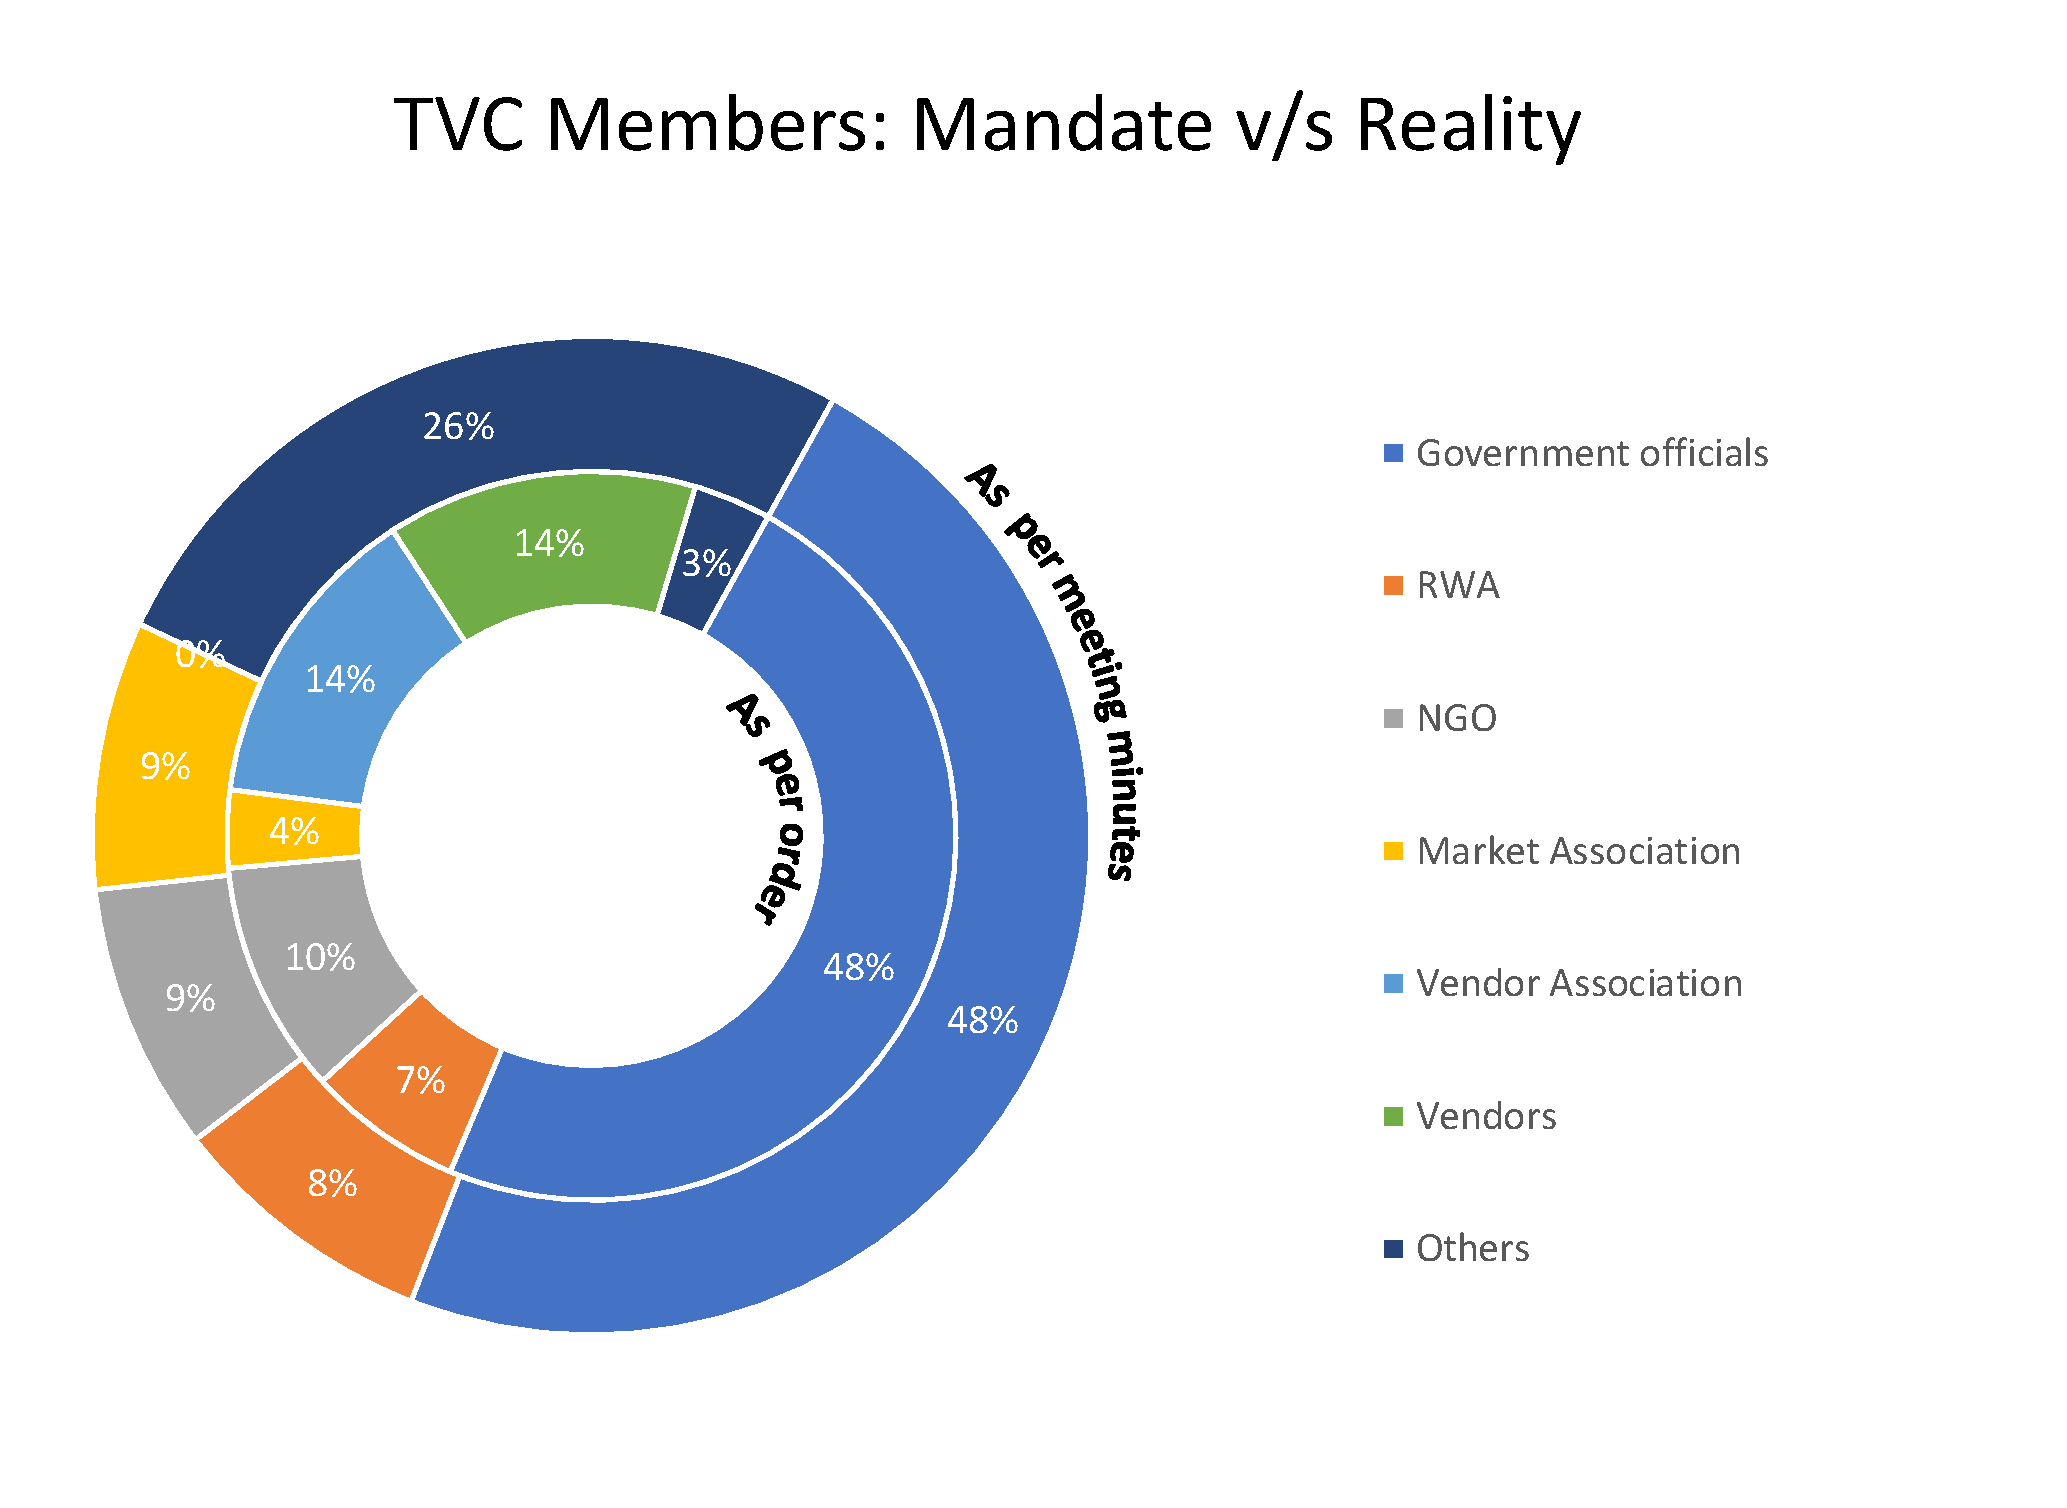
\includegraphics[height=0.6\textwidth]{mandatevsreality.pdf}
%\end{figure}

	\begin{figure}[h]
		%Do not try to scale figure in .tex or you loose font size consistency
		%\hspace*{-3cm}
		%The code to input the plot is extremely simple
		% Created by tikzDevice version 0.12 on 2019-02-12 15:48:00
% !TEX encoding = UTF-8 Unicode
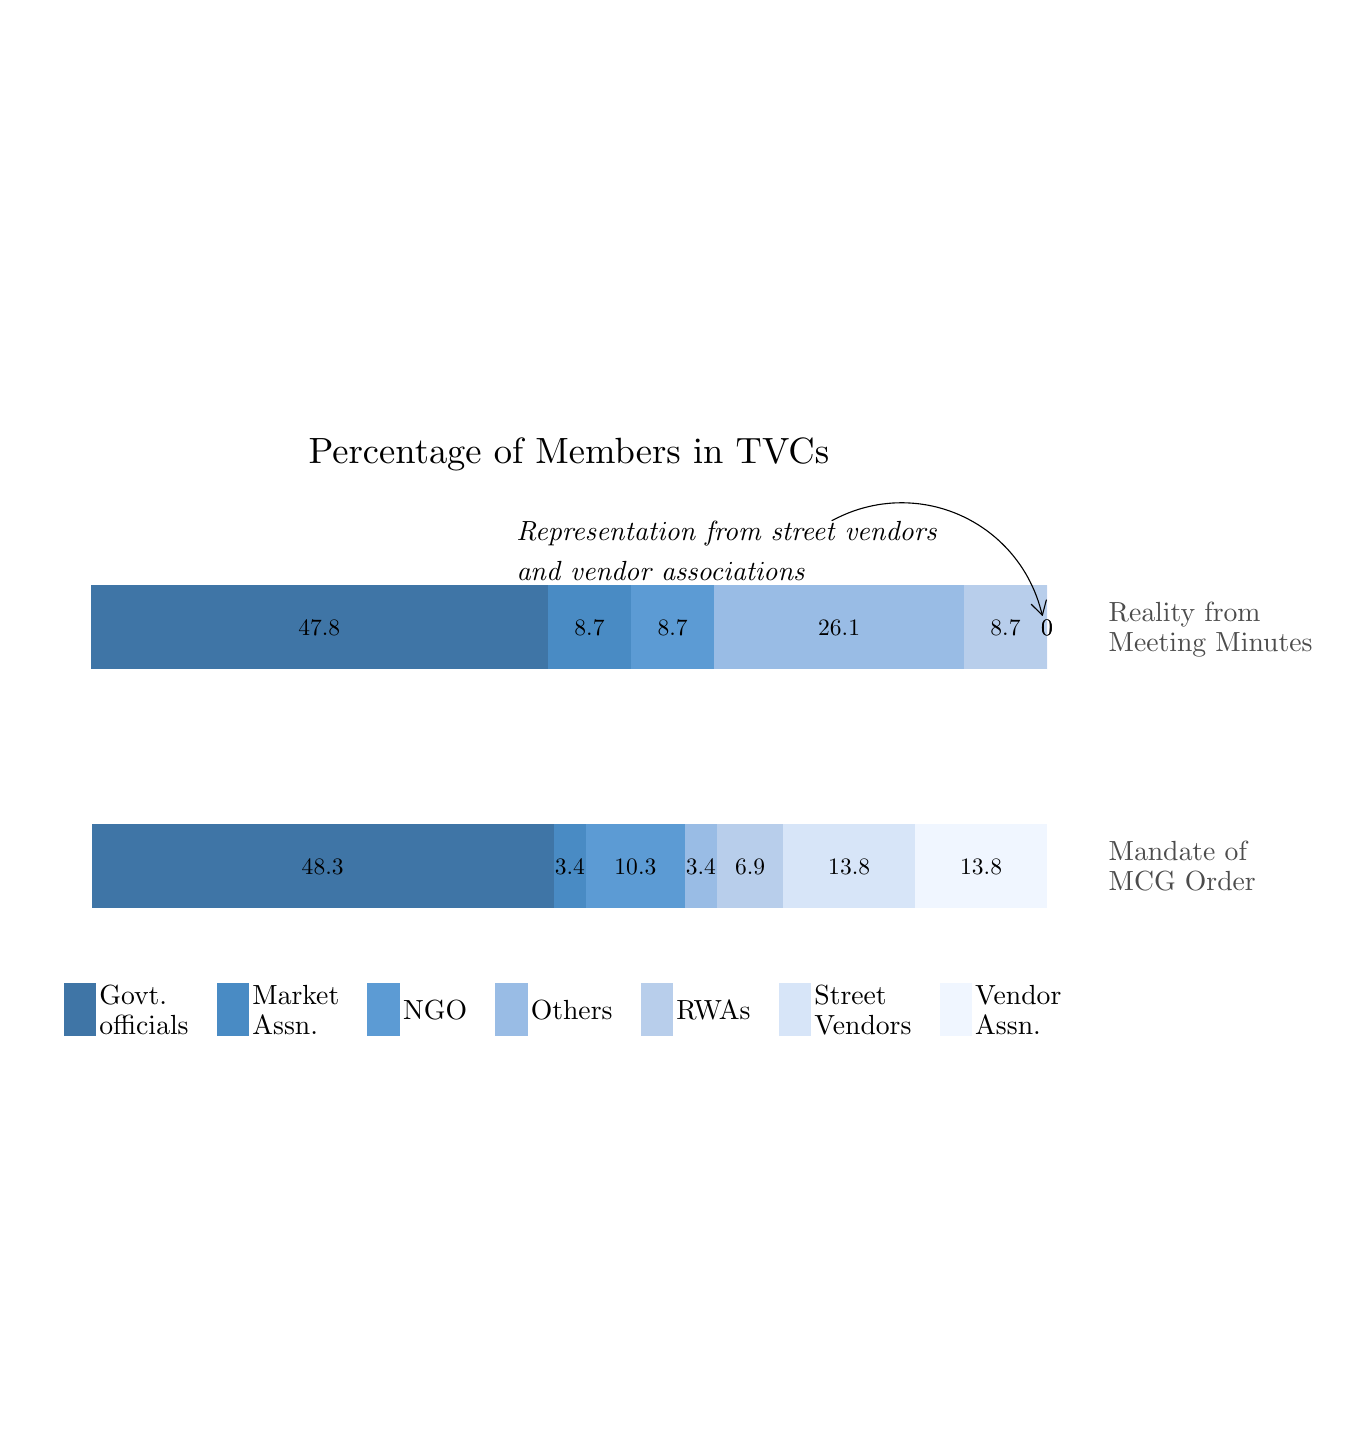
\begin{tikzpicture}[x=1pt,y=1pt]
\definecolor{fillColor}{RGB}{255,255,255}
\path[use as bounding box,fill=fillColor,fill opacity=0.00] (0,0) rectangle (469.75,505.89);
\begin{scope}
\path[clip] (  0.00,142.76) rectangle (469.75,363.13);
\definecolor{drawColor}{RGB}{255,255,255}
\definecolor{fillColor}{RGB}{255,255,255}

\path[draw=drawColor,line width= 0.6pt,line join=round,line cap=round,fill=fillColor] (  0.00,142.76) rectangle (469.76,363.13);
\end{scope}
\begin{scope}
\path[clip] (  5.50,151.01) rectangle (385.66,341.09);
\definecolor{fillColor}{RGB}{240,246,255}

\path[fill=fillColor] (320.68,187.73) rectangle (368.38,217.97);
\definecolor{fillColor}{RGB}{215,229,248}

\path[fill=fillColor] (272.99,187.73) rectangle (320.68,217.97);
\definecolor{fillColor}{RGB}{184,206,235}

\path[fill=fillColor] (249.15,187.73) rectangle (272.99,217.97);
\definecolor{fillColor}{RGB}{153,188,229}

\path[fill=fillColor] (237.40,187.73) rectangle (249.15,217.97);
\definecolor{fillColor}{RGB}{92,155,212}

\path[fill=fillColor] (201.80,187.73) rectangle (237.40,217.97);
\definecolor{fillColor}{RGB}{73,139,196}

\path[fill=fillColor] (190.05,187.73) rectangle (201.80,217.97);
\definecolor{fillColor}{RGB}{63,117,166}

\path[fill=fillColor] ( 23.13,187.73) rectangle (190.05,217.97);
\definecolor{fillColor}{RGB}{184,206,235}

\path[fill=fillColor] (338.31,274.13) rectangle (368.38,304.37);
\definecolor{fillColor}{RGB}{153,188,229}

\path[fill=fillColor] (248.11,274.13) rectangle (338.31,304.37);
\definecolor{fillColor}{RGB}{92,155,212}

\path[fill=fillColor] (218.04,274.13) rectangle (248.11,304.37);
\definecolor{fillColor}{RGB}{73,139,196}

\path[fill=fillColor] (187.98,274.13) rectangle (218.04,304.37);
\definecolor{fillColor}{RGB}{63,117,166}

\path[fill=fillColor] ( 22.78,274.13) rectangle (187.98,304.37);
\definecolor{fillColor}{RGB}{240,246,255}

\path[fill=fillColor] (368.38,274.13) rectangle (368.38,304.37);
\definecolor{fillColor}{RGB}{215,229,248}

\path[fill=fillColor] (368.38,274.13) rectangle (368.38,304.37);
\definecolor{drawColor}{RGB}{0,0,0}

\node[text=drawColor,anchor=base,inner sep=0pt, outer sep=0pt, scale=  0.85] at (344.53,199.91) {13.8};

\node[text=drawColor,anchor=base,inner sep=0pt, outer sep=0pt, scale=  0.85] at (296.84,199.91) {13.8};

\node[text=drawColor,anchor=base,inner sep=0pt, outer sep=0pt, scale=  0.85] at (261.07,199.91) {6.9};

\node[text=drawColor,anchor=base,inner sep=0pt, outer sep=0pt, scale=  0.85] at (243.27,199.91) {3.4};

\node[text=drawColor,anchor=base,inner sep=0pt, outer sep=0pt, scale=  0.85] at (219.60,199.91) {10.3};

\node[text=drawColor,anchor=base,inner sep=0pt, outer sep=0pt, scale=  0.85] at (195.92,199.91) {3.4};

\node[text=drawColor,anchor=base,inner sep=0pt, outer sep=0pt, scale=  0.85] at (106.59,199.91) {48.3};

\node[text=drawColor,anchor=base,inner sep=0pt, outer sep=0pt, scale=  0.85] at (353.34,286.31) {8.7};

\node[text=drawColor,anchor=base,inner sep=0pt, outer sep=0pt, scale=  0.85] at (293.21,286.31) {26.1};

\node[text=drawColor,anchor=base,inner sep=0pt, outer sep=0pt, scale=  0.85] at (233.08,286.31) {8.7};

\node[text=drawColor,anchor=base,inner sep=0pt, outer sep=0pt, scale=  0.85] at (203.01,286.31) {8.7};

\node[text=drawColor,anchor=base,inner sep=0pt, outer sep=0pt, scale=  0.85] at (105.38,286.31) {47.8};

\node[text=drawColor,anchor=base,inner sep=0pt, outer sep=0pt, scale=  0.85] at (368.38,286.31) {0};

\node[text=drawColor,anchor=base,inner sep=0pt, outer sep=0pt, scale=  0.85] at (368.38,286.31) {0};

\path[draw=drawColor,line width= 0.4pt,line join=round,line cap=round] (290.62,327.79) --
	(290.83,327.89) --
	(291.80,328.37) --
	(293.00,328.95) --
	(293.97,329.41) --
	(294.77,329.77) --
	(295.56,330.11) --
	(296.43,330.47) --
	(297.35,330.83) --
	(298.23,331.15) --
	(299.05,331.44) --
	(299.87,331.71) --
	(300.77,331.99) --
	(301.71,332.26) --
	(302.62,332.51) --
	(303.46,332.72) --
	(304.30,332.92) --
	(305.22,333.12) --
	(306.19,333.31) --
	(307.11,333.48) --
	(307.96,333.62) --
	(308.82,333.74) --
	(309.75,333.85) --
	(310.73,333.96) --
	(311.67,334.04) --
	(312.53,334.11) --
	(313.40,334.15) --
	(314.34,334.19) --
	(315.32,334.20) --
	(316.26,334.21) --
	(317.13,334.19) --
	(317.99,334.16) --
	(318.93,334.11) --
	(319.91,334.04) --
	(320.85,333.96) --
	(321.71,333.87) --
	(322.57,333.77) --
	(323.50,333.63) --
	(324.47,333.48) --
	(325.40,333.32) --
	(326.25,333.15) --
	(327.09,332.97) --
	(328.01,332.76) --
	(328.96,332.52) --
	(329.87,332.27) --
	(330.70,332.03) --
	(331.53,331.78) --
	(332.42,331.48) --
	(333.35,331.16) --
	(334.24,330.83) --
	(335.04,330.52) --
	(335.84,330.20) --
	(336.71,329.82) --
	(337.61,329.42) --
	(338.46,329.02) --
	(339.23,328.64) --
	(340.00,328.24) --
	(340.83,327.79) --
	(341.69,327.31) --
	(342.50,326.84) --
	(343.24,326.39) --
	(343.97,325.93) --
	(344.76,325.41) --
	(345.57,324.85) --
	(346.34,324.31) --
	(347.03,323.80) --
	(347.72,323.27) --
	(348.46,322.69) --
	(349.22,322.06) --
	(349.94,321.45) --
	(350.58,320.88) --
	(351.22,320.30) --
	(351.90,319.65) --
	(352.61,318.96) --
	(353.27,318.29) --
	(353.86,317.66) --
	(354.45,317.02) --
	(355.07,316.32) --
	(355.71,315.57) --
	(356.31,314.84) --
	(356.84,314.17) --
	(357.37,313.48) --
	(357.93,312.72) --
	(358.50,311.92) --
	(359.03,311.14) --
	(359.51,310.42) --
	(359.97,309.69) --
	(360.46,308.89) --
	(360.96,308.04) --
	(361.42,307.22) --
	(361.83,306.46) --
	(362.22,305.69) --
	(362.64,304.84) --
	(363.06,303.95) --
	(363.45,303.10) --
	(363.79,302.30) --
	(364.12,301.50) --
	(364.46,300.63) --
	(364.80,299.70) --
	(365.11,298.81) --
	(365.38,297.99) --
	(365.64,297.16) --
	(365.94,296.13) --
	(366.30,294.84) --
	(366.58,293.81) --
	(366.65,293.57);

\path[draw=drawColor,line width= 0.4pt,line join=round,line cap=round] (362.60,297.57) --
	(366.65,293.57) --
	(368.09,299.08);
\end{scope}
\begin{scope}
\path[clip] (  5.50,151.01) rectangle (385.66,341.09);
\definecolor{drawColor}{RGB}{0,0,0}

\node[text=drawColor,anchor=base west,inner sep=0pt, outer sep=0pt, scale=  1.00] at (176.57,320.59) {\itshape Representation from street vendors};

\node[text=drawColor,anchor=base west,inner sep=0pt, outer sep=0pt, scale=  1.00] at (176.57,306.19) {\itshape and vendor associations};
\end{scope}
\begin{scope}
\path[clip] (  0.00,  0.00) rectangle (469.75,505.89);
\definecolor{drawColor}{gray}{0.30}

\node[text=drawColor,anchor=base west,inner sep=0pt, outer sep=0pt, scale=  1.00] at (390.61,204.81) {Mandate of};

\node[text=drawColor,anchor=base west,inner sep=0pt, outer sep=0pt, scale=  1.00] at (390.61,194.01) {MCG Order};

\node[text=drawColor,anchor=base west,inner sep=0pt, outer sep=0pt, scale=  1.00] at (390.61,291.21) {Reality from};

\node[text=drawColor,anchor=base west,inner sep=0pt, outer sep=0pt, scale=  1.00] at (390.61,280.41) {Meeting Minutes};
\end{scope}
\begin{scope}
\path[clip] (  0.00,  0.00) rectangle (469.75,505.89);
\definecolor{fillColor}{RGB}{255,255,255}

\path[fill=fillColor] ( 12.83,141.20) rectangle (393.53,160.83);
\end{scope}
\begin{scope}
\path[clip] (  0.00,  0.00) rectangle (469.75,505.89);
\definecolor{drawColor}{RGB}{255,255,255}
\definecolor{fillColor}{gray}{0.95}

\path[draw=drawColor,line width= 5.7pt,line join=round,line cap=round,fill=fillColor] ( 12.83,141.20) rectangle ( 24.88,160.83);
\end{scope}
\begin{scope}
\path[clip] (  0.00,  0.00) rectangle (469.75,505.89);
\definecolor{fillColor}{RGB}{63,117,166}

\path[fill=fillColor] ( 13.02,141.39) rectangle ( 24.69,160.64);
\end{scope}
\begin{scope}
\path[clip] (  0.00,  0.00) rectangle (469.75,505.89);
\definecolor{drawColor}{RGB}{255,255,255}
\definecolor{fillColor}{gray}{0.95}

\path[draw=drawColor,line width= 5.7pt,line join=round,line cap=round,fill=fillColor] ( 68.15,141.20) rectangle ( 80.19,160.83);
\end{scope}
\begin{scope}
\path[clip] (  0.00,  0.00) rectangle (469.75,505.89);
\definecolor{fillColor}{RGB}{73,139,196}

\path[fill=fillColor] ( 68.34,141.39) rectangle ( 80.01,160.64);
\end{scope}
\begin{scope}
\path[clip] (  0.00,  0.00) rectangle (469.75,505.89);
\definecolor{drawColor}{RGB}{255,255,255}
\definecolor{fillColor}{gray}{0.95}

\path[draw=drawColor,line width= 5.7pt,line join=round,line cap=round,fill=fillColor] (122.60,141.20) rectangle (134.65,160.83);
\end{scope}
\begin{scope}
\path[clip] (  0.00,  0.00) rectangle (469.75,505.89);
\definecolor{fillColor}{RGB}{92,155,212}

\path[fill=fillColor] (122.79,141.39) rectangle (134.46,160.64);
\end{scope}
\begin{scope}
\path[clip] (  0.00,  0.00) rectangle (469.75,505.89);
\definecolor{drawColor}{RGB}{255,255,255}
\definecolor{fillColor}{gray}{0.95}

\path[draw=drawColor,line width= 5.7pt,line join=round,line cap=round,fill=fillColor] (168.77,141.20) rectangle (180.81,160.83);
\end{scope}
\begin{scope}
\path[clip] (  0.00,  0.00) rectangle (469.75,505.89);
\definecolor{fillColor}{RGB}{153,188,229}

\path[fill=fillColor] (168.95,141.39) rectangle (180.62,160.64);
\end{scope}
\begin{scope}
\path[clip] (  0.00,  0.00) rectangle (469.75,505.89);
\definecolor{drawColor}{RGB}{255,255,255}
\definecolor{fillColor}{gray}{0.95}

\path[draw=drawColor,line width= 5.7pt,line join=round,line cap=round,fill=fillColor] (221.33,141.20) rectangle (233.38,160.83);
\end{scope}
\begin{scope}
\path[clip] (  0.00,  0.00) rectangle (469.75,505.89);
\definecolor{fillColor}{RGB}{184,206,235}

\path[fill=fillColor] (221.52,141.39) rectangle (233.19,160.64);
\end{scope}
\begin{scope}
\path[clip] (  0.00,  0.00) rectangle (469.75,505.89);
\definecolor{drawColor}{RGB}{255,255,255}
\definecolor{fillColor}{gray}{0.95}

\path[draw=drawColor,line width= 5.7pt,line join=round,line cap=round,fill=fillColor] (271.23,141.20) rectangle (283.28,160.83);
\end{scope}
\begin{scope}
\path[clip] (  0.00,  0.00) rectangle (469.75,505.89);
\definecolor{fillColor}{RGB}{215,229,248}

\path[fill=fillColor] (271.42,141.39) rectangle (283.09,160.64);
\end{scope}
\begin{scope}
\path[clip] (  0.00,  0.00) rectangle (469.75,505.89);
\definecolor{drawColor}{RGB}{255,255,255}
\definecolor{fillColor}{gray}{0.95}

\path[draw=drawColor,line width= 5.7pt,line join=round,line cap=round,fill=fillColor] (329.35,141.20) rectangle (341.40,160.83);
\end{scope}
\begin{scope}
\path[clip] (  0.00,  0.00) rectangle (469.75,505.89);
\definecolor{fillColor}{RGB}{240,246,255}

\path[fill=fillColor] (329.54,141.39) rectangle (341.21,160.64);
\end{scope}
\begin{scope}
\path[clip] (  0.00,  0.00) rectangle (469.75,505.89);
\definecolor{drawColor}{RGB}{0,0,0}

\node[text=drawColor,anchor=base west,inner sep=0pt, outer sep=0pt, scale=  1.00] at ( 25.88,152.97) {Govt.};

\node[text=drawColor,anchor=base west,inner sep=0pt, outer sep=0pt, scale=  1.00] at ( 25.88,142.17) {officials};
\end{scope}
\begin{scope}
\path[clip] (  0.00,  0.00) rectangle (469.75,505.89);
\definecolor{drawColor}{RGB}{0,0,0}

\node[text=drawColor,anchor=base west,inner sep=0pt, outer sep=0pt, scale=  1.00] at ( 81.19,152.97) {Market};

\node[text=drawColor,anchor=base west,inner sep=0pt, outer sep=0pt, scale=  1.00] at ( 81.19,142.17) {Assn.};
\end{scope}
\begin{scope}
\path[clip] (  0.00,  0.00) rectangle (469.75,505.89);
\definecolor{drawColor}{RGB}{0,0,0}

\node[text=drawColor,anchor=base west,inner sep=0pt, outer sep=0pt, scale=  1.00] at (135.65,147.57) {NGO};
\end{scope}
\begin{scope}
\path[clip] (  0.00,  0.00) rectangle (469.75,505.89);
\definecolor{drawColor}{RGB}{0,0,0}

\node[text=drawColor,anchor=base west,inner sep=0pt, outer sep=0pt, scale=  1.00] at (181.81,147.57) {Others};
\end{scope}
\begin{scope}
\path[clip] (  0.00,  0.00) rectangle (469.75,505.89);
\definecolor{drawColor}{RGB}{0,0,0}

\node[text=drawColor,anchor=base west,inner sep=0pt, outer sep=0pt, scale=  1.00] at (234.38,147.57) {RWAs};
\end{scope}
\begin{scope}
\path[clip] (  0.00,  0.00) rectangle (469.75,505.89);
\definecolor{drawColor}{RGB}{0,0,0}

\node[text=drawColor,anchor=base west,inner sep=0pt, outer sep=0pt, scale=  1.00] at (284.28,152.97) {Street};

\node[text=drawColor,anchor=base west,inner sep=0pt, outer sep=0pt, scale=  1.00] at (284.28,142.17) {Vendors};
\end{scope}
\begin{scope}
\path[clip] (  0.00,  0.00) rectangle (469.75,505.89);
\definecolor{drawColor}{RGB}{0,0,0}

\node[text=drawColor,anchor=base west,inner sep=0pt, outer sep=0pt, scale=  1.00] at (342.40,152.97) {Vendor};

\node[text=drawColor,anchor=base west,inner sep=0pt, outer sep=0pt, scale=  1.00] at (342.40,142.17) {Assn.};
\end{scope}
\begin{scope}
\path[clip] (  0.00,  0.00) rectangle (469.75,505.89);
\definecolor{drawColor}{RGB}{0,0,0}

\node[text=drawColor,anchor=base,inner sep=0pt, outer sep=0pt, scale=  1.32] at (195.58,348.54) {Percentage of Members in TVCs};
\end{scope}
\end{tikzpicture}

		%Captions and Labels can be used since this is a figure environment
		\vspace{-2cm}
		%\caption{Sample output from tikzDevice}
		\label{plot:test}
	\end{figure}
	


\subsubsection*{Low Vendor Representation at TVC Meetings Resulting in Biased Decisions}
\addcontentsline{toc}{subsubsection}{Low Vendor Representation at TVC Meetings Resulting in Biased Decisions}

The mandated list of TVC members of the local authority’s includes four vendors; however, the minutes of the meeting held on 21 August 2018 show zero representation from vendors (Appendix \ref{appendix: TVC members}). The meeting had 23 signatories with no vendors, but the content of the minutes referred to the presence of three vendor representatives. When asked to clarify, one of the vendor representatives explained that the discrepancy was due to the unwillingness of members to ratify minutes, given differences of opinion.

Separately, we also reached out to 15 of the 23 signatories to verify their presence at the meeting. Three denied being a part of any such meeting. One NGO member, on the condition of anonymity, mentioned that he was only present as he is `friends with the City Project Officer'.{\footnote{Respondent number 15, 21 and 22 from the list in Appendix \ref{appendix: TVC members} denied being a part of the TVC; one, being a representative from the market welfare association and second, the ad-hoc pradhan of Sector 14.}

\subsubsection*{Disagreement Between Government Officials and Vendors on Vending Sites}
\addcontentsline{toc}{subsubsection}{Disagreement Between Government Officials and Vendors on Vending Sites}

Vendor representatives expressed disagreement with the TVC’s approach on withdrawal of two vending sites from Sector 14.

\begin{wrapfigure}{r}{0.55\textwidth}
\vspace{-10pt}
\hspace{-20pt}
\centering
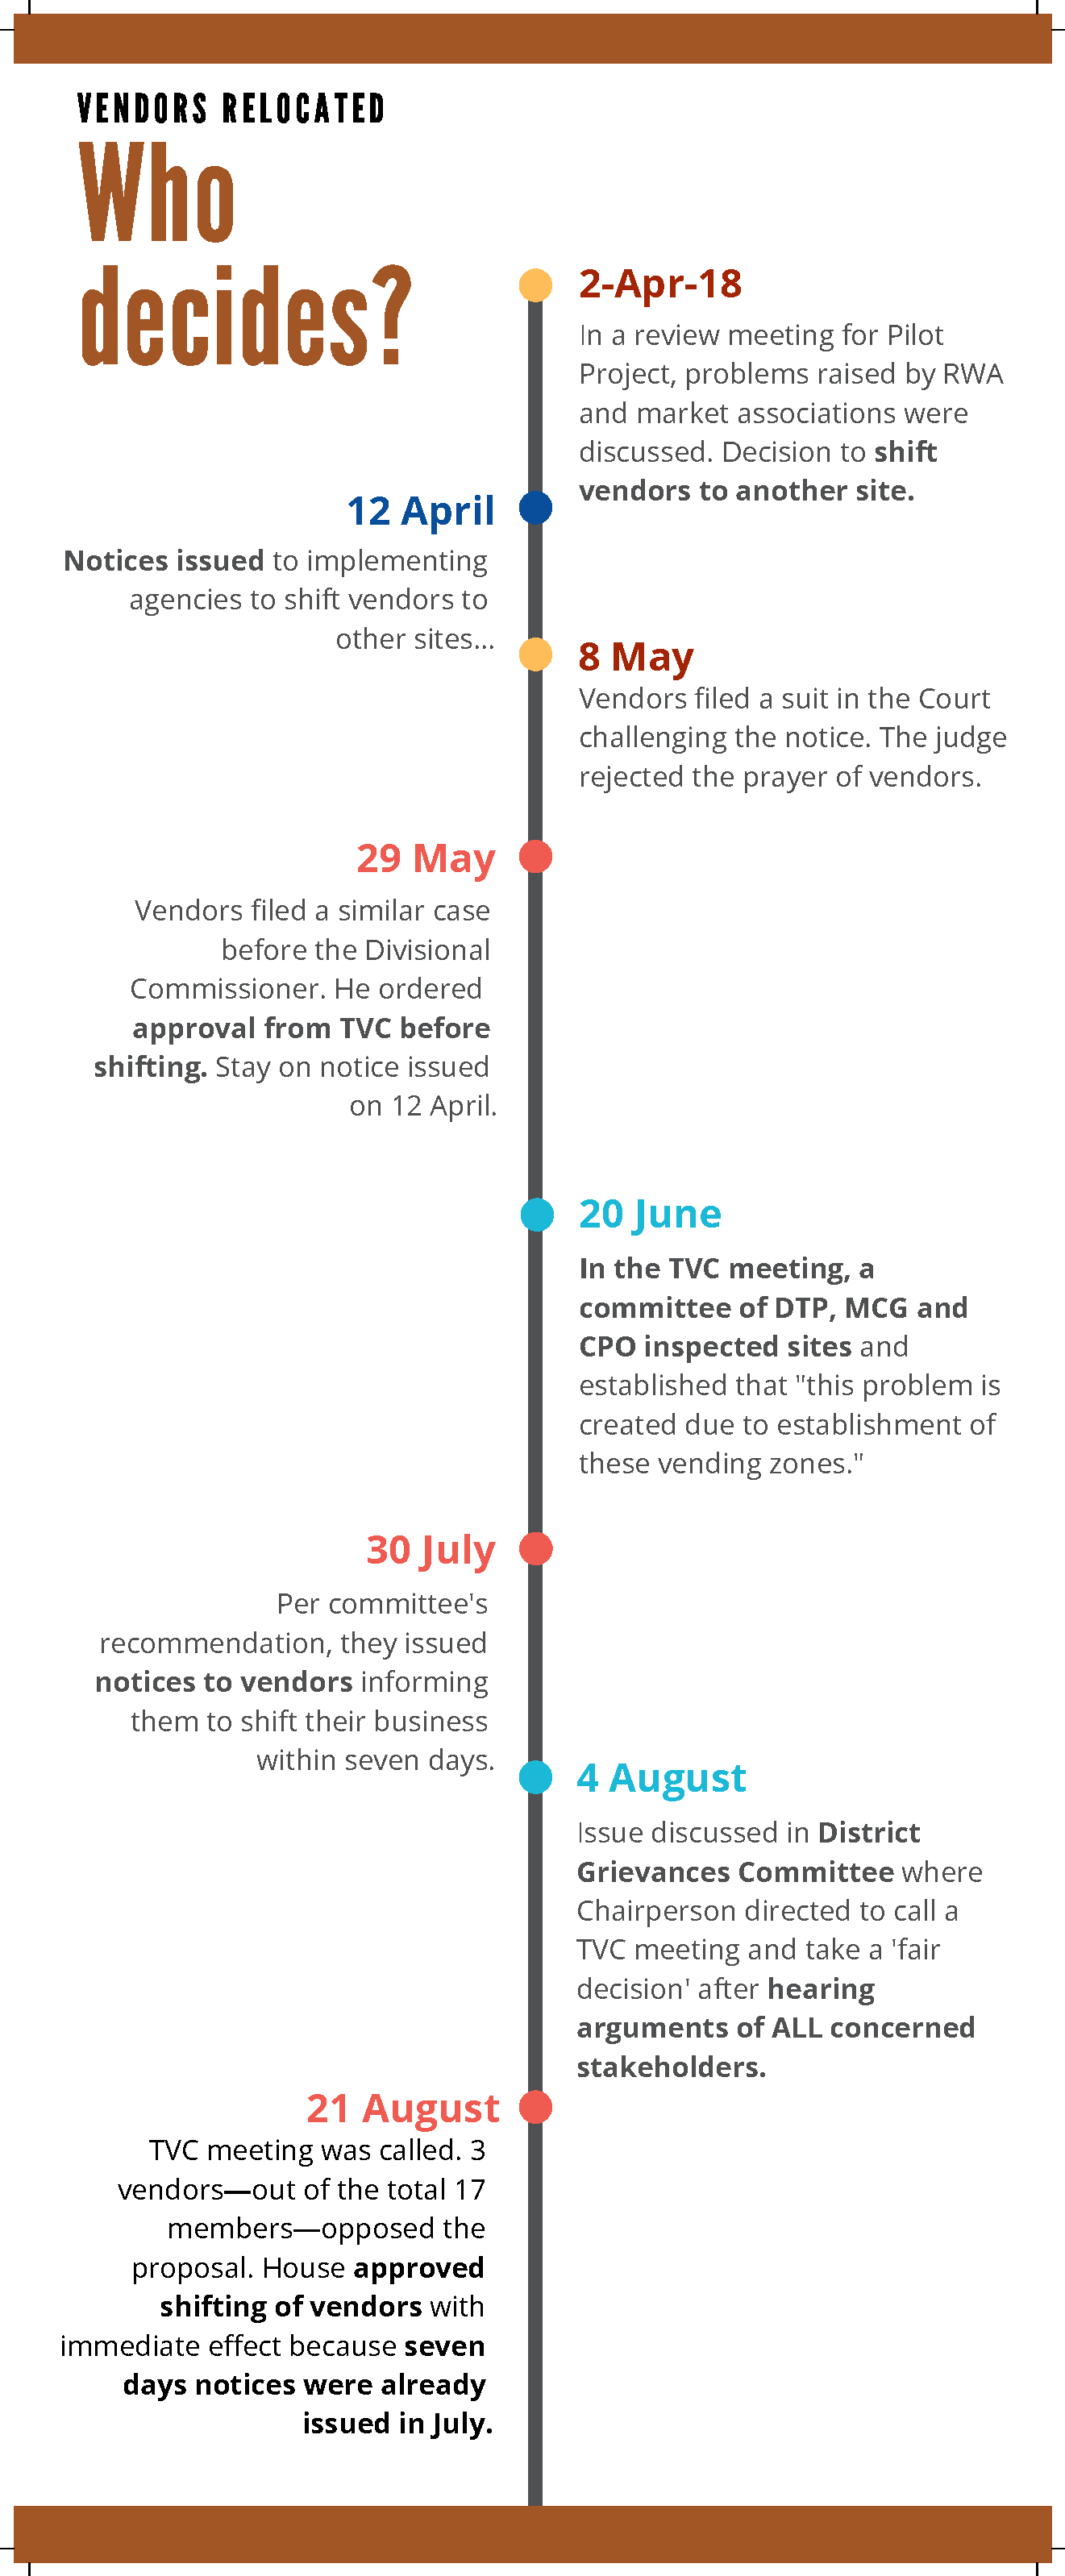
\includegraphics[height=17.6cm]{WhoDecides.pdf}
\vspace{-40pt}
\end{wrapfigure}

The meeting on 21 August 2018 was called to `take fair decision … regarding shifting of vending zones after hearing arguments of all concerned parties/stakeholders'. This was after three complaints by vendors to different authorities for reconsideration of the decision to withdraw sites. Out of the 17 members who voted on the decision, only 3 opposed. All three members were representatives of vendors. The minutes conclude by referring to the `democratically expressed views of the majority' and issued an order to shift vendors with `immediate effect'.

This example of the withdrawal of two sites from Sector 14 reflects how vendors may be overpowered easily in the absence of sufficient representation and a genuine will to formalise vendors. The effort here, it seems, is to secure majority agreement to a pre-decided position. The meeting minutes repeatedly referred to problems caused by vendors but were silent on the argument raised by vendors.

In Gurugram, the MCG has earmarked 49 vending zones—37 in September and 12 in October 2017. Some vendors registered to operate in the earmarked vending zone moved since the appointed vending zone was not in the vicinity of a residential area and experienced low levels of pedestrian footfall. Moving street vendors to `off-street locations is relatively easy, but moving their customers to those locations is much more difficult. When customers fail to follow, vendors have little choice but to return to the streets' \parencite{bromleypaper}.

These two examples raise questions on the willingness of municipal officials to include vendors in critical decisions. How are vending zones earmarked?\footnote{Meeting minutes of 21 August 2018 state: `as per approved layout plan of Haryana Urban Development Authority (HUDA), the site is earmarked for Parking and other is earmarked as Cycle Stand… prior to development of vending zones, permission was not obtained from Town and Country Planning Department to change use of sites as vending zone'.} In the case of disputes or conflicts, how are decisions made? Is there a structured channel of dispute resolution? How are the street vendors or their interests incorporated in such decisions?





Although the Act opens channels and creates a super structure for negotiation between government and civil society, the devil lies in the detail. The suppression or protection of vendors will depend on the quality of regulations proposed by the local authority. The Act requires the plan for street vending to recognise the existing markets where buyers and sellers congregate. For any spatial planning exercise to be successful, it must take into consideration the commercial viability of vending sites. A thoughtful consideration of the existing patterns of vending is necessary to ensure that the demarcation of zones does not become a futile exercise.


\subsubsection*{Contracting out TVC functions}
\addcontentsline{toc}{subsubsection}{Contracting out TVC functions}

The Act and the state government’s rules provide for the TVC to `temporarily associate itself with any person for their assistance or advice in carrying out provisions of the Act'. When MCG invited enterprises to participate in the pilot project, eight showed interest, and four were shortlisted between 2015 and 2016. The local body allotted sectors to the four shortlisted firms, SSSPL, Leo Mediacom, Egmac Capital and National Association of Street Vendors of India (NASVI), through draw of lots or a consensus.

Some of the tasks delegated to the private firms include:
\begin{itemize}
\item Spatial planning taking into account natural markets, weekend markets, weekly haats, and night bazaars;
\item Demarcation of vending sites;
\item Design of carts to optimise space, keeping `aesthetics' into consideration;
\item Exhibit regulation and management of vendors;
\item Proposal for solid waste management;
\item Enumeration in allocated zones and;
\item Monitoring food adulteration and compliance with Food Safety and Standards Authority of India norms.
\end{itemize}

Two years since the contract was signed, SSSPL has enumerated and registered vendors, and distributed carts in two out of seven allocated areas. In this section, we raise some questions on the enumeration exercise and fee imposed on vendors for the new carts.

\paragraph*{Multiple Surveys, Multiple Identities?} 
%\addcontentsline{toc}{paragraph}{Multiple Surveys, Multiple Identities?}

In Gurugram, the enumeration of vendors was first done in 2014. The exercise identified more than 14,000 vendors in all 35 wards. In 2016, the three shortlisted private firms re-surveyed the sites to ensure that all vendors in the sectors allocated to them were enlisted. In 2018, the Haryana government started a new exercise that aspired to cover vendors of the whole state. \\

\begin{mdframed}[backgroundcolor=gray!20]
In one of our interviews with vendors, an unregistered vendor stated that in June 2018, police authorities seized her cart goods on the grounds of it being a no-vending zone. She has been vending for eight years at MG Road metro station; however, she was excluded in the enumeration exercise of 2014. Section 3.3 of the Act mandates that no street vendor shall be evicted or relocated till the enumeration exercise and issuance of vending certificates are complete. Moreover, the Act prohibits declaration of a no-vending zone before the completion of the enumeration and formulation of the street vending plan. While she was allowed to reclaim her goods, she still can not vend for the fear of being evicted or harassed. In the absence of a one-stop grievance redressal committee, many vendors like her struggle to find the right platform to voice their concerns.
\end{mdframed}

The RTI response from Government of Haryana, noted the identification of 18,670 vendors in Gurugram and the status of enumeration exercise as ‘ongoing’. By when will the survey be complete? What is the approach for conducting these surveys? How do these exercises by different enterprises guarantee identification of all vendors?

Streets are dynamic. Some vendors are stationary, some mobile. Even stationary vendors operate from multiple locations depending on the time of the year or day. Some operate full-time, some part time and others seasonally. The manner in which the local authority and other stakeholders accommodate the fluctuations is crucial for the exhaustive and accommodative registration of vendors.

\paragraph*{Fees and Fines: What Does the Vendor Earn and Pay?}
%\addcontentsline{toc}{subsubsection}{Fees and Fines: What Does the Vendor Earn and Pay?}


\begin{wrapfigure}{l}{0.61\textwidth}
\vspace{0pt}

\centering
\includegraphics[width=0.60\textwidth]{"ggncart".png}

\end{wrapfigure}

The scheme for street vendors must provide for `the manner of collecting ...vending fees, maintenance charges and penalties for registration'.

Vendors in Gurugram, under the new policy, pay a one-time cart fee of Rs 85,000 to 1.5 lakh. The TVC meeting held in June 2016 discussed financing of the carts. The local authority refused to grant advertising rights to private enterprises who were willing to provide carts free of cost, if such rights were accorded. Private parties alternatively offered to issue loans to vendors who cannot self-finance. Vendor representatives agreed stating that `street vendors are being harassed at multiple levels and they are willing to invest in anything which renders them recognition and security of tenure at a given location'.

The minutes did not give the rationale for the rejection of advertising rights. One of the key innovations of a similar public-private partnership in Bhubaneswar in 2006 was to obtain advertising firms to partly finance the carts.

In addition to the cart fee, vendors pay a monthly maintenance fee. SSSPL, for example, charges Rs 1,500. The MCG and the enterprise share the maintenance fee in the ratio of 1:2. The MCG generates an average revenue of Rs 10 to 12 lakh annually from this.

The costs imposed on vendors and its impact are pertinent subjects but outside the scope of this study. Some of the questions for further research are: Are vendors able to afford the `aesthetic' carts? How many vendors have been issued loans? What if vendors fail to replay? How are the funds generated through the collection of maintenance and other fees used?

\subsubsection*{No Mechanism for Grievance Redressal Despite Piling Complaints}
\addcontentsline{toc}{subsubsection}{No Mechanism for Grievance Redressal Despite Piling Complaints}

Section 20.1 of the Act requires the appropriate government to constitute a grievance redressal committee chaired by an ex-civil judge or judicial magistrate. In Gurugram, the City Project Officer personally attends to disputes.

As affirmed by the private enterprise, the lack of a grievance redressal committee makes it difficult for vendors to report harassment. The representative of the enterprise showed us a file full of complaints addressed to the MCG. There is no information about the redressal status of these complaints.

In the TVC meeting held on 21 August 2018, the Assistant Commissioner of Police `assured that the police personnel will not harass the vendors unnecessarily and if any instance is noticed by the vendors/association, the same should be brought to the notice of Deputy Commissioner of Police (DCP) (Headquarters)/DCP (Traffic)'. But during our interviews vendor association representatives were quick to point out that vendors continue to be harassed and evicted—the police levies varying challan payments worth Rs 1,200 to Rs 5,000 and the MCG charges Rs 5,000 to Rs 10,000 for failure in maintaining cleanliness. The Police officials also frequently seized goods, reclaiming which was a tedious and lengthy process.

In the absence of a clear channel, how does the vendor solve the problems? What is the approach to curtailing evictions and other difficulties of vendors, until the formation of a grievance redressal committee? How will decisions be unbiased given that those vendors seek protection from—the police and municipality—are the ones tasked with protecting them?

%\subsection{Delhi: The Fight for Legitimacy Continues}
\subsection*{Delhi: The Fight for Legitimacy Continues}
\addcontentsline{toc}{subsection}{Delhi: The Fight for Legitimacy Continues}


The National Capital Region is one of the richest areas in the country. Delhi, the centre of the region, boasts per capita incomes three times the national average. Yet, 17 lakh people in the city live below the poverty line \parencite{delhireport}. There are close to 3,00,000 street vendors in Delhi \parencite{sewapaper} but official (and outdated) lists only recognise half of these. 

Delhi makes for a unique case where vendors face resistance from both, the administration and the judiciary. An analysis of case laws shows how Delhi’s vendors are frequently disfavoured. More than 3 years after the Act, the High Court of Delhi continues to base eviction decisions on the pre-2014 legal status of vendors and uphold the old demarcation of vending zones. Between January 2017 and September 2018, vendor petitioners challenged evictions 22 times, of which the High Court of Delhi ruled against vendors in 14 cases. The scheme framed by the government has also been criticised for over-regulation by different vendor interest groups and advocates. 

We studied why the schemes and rules remain contentious, the new TVCs formed and their functioning. This case study is based on a review of pertinent case laws and six interviews with TVC members, one government official, TVC members in NDMC, and an advocate for vendor rights. While we reached out to TVCs in all four municipal zones, we only secured interviews from the New Delhi Municipal Council (NDMC). The NDMC governs the seat of the power of the Union of India and covers areas such as the Central Secretariat and Connaught Place. 

The list of interviewees included the following:
\begin{itemize}[nosep]
\item TVC members:
\begin{itemize}
\item NGO: Indo-Global Social Service Society
\item Community-based Organization: Janpahal
\item One elected vendor

\item Representative from one vendor association: National Hawkers Federation
\end{itemize}
\item Non-TVC members:
\begin{itemize}
\item An NDMC official in the `TVC Department' who attends TVC meetings but is not a member
\item Indira Unninayar, Advocate, Supreme Court and Delhi High Court
\end{itemize}
\end{itemize}

\subsubsection*{The Scheme Focused More on Regulation, Less on Protection}
\addcontentsline{toc}{subsubsection}{The Scheme Focused More on Regulation, Less on Protection}

The Government of NCT of Delhi notified the \href{http://mohua.gov.in/upload/uploadfiles/files/6(2).pdf}{Delhi Street Vendors Scheme} in September 2015 and again in January 2016. Both schemes were contested by vendor interest groups \parencite{tirkeynews}. The 2015 scheme had several provisions that were excessive and against the mandate of the Act. Although the Act prohibits overcrowding and sanitary concerns basis for demarcating no-vending zones, the Delhi scheme included `traffic congestion' and `cleanliness.` Moreover, the scheme introduced requirements for no-objection certificates from the Resident Welfare Associations and Market Associations in defining vending zones. This defeats the purpose of participatory governance with vendor representation because zones can be demarcated solely with the approval of residents and shop owners. 

Further, the Delhi’s scheme had bright-line rules such as `space for vending shall be 6×8 feet', `height shall not be more than 3 feet', and `vendors shall not make any noise for attracting the public or customers'. The scheme also prohibited cooking and vending around places of worship, educational institutions, hospitals or railway stations. The vending time was restricted from `sunrise to sunset'. 

Vendor interest groups challenged the 2016 scheme in court. The petitioner argued that the scheme was prepared without any consultation with the TVCs. The Court stayed the order and held that the scheme be revised and enacted only after TVC was formed (Janodaya Ekta Samiti v Govt. of NCT of Delhi and Ors.). 

This instance has a bearing on all other states that have formed rules and schemes without constituting TVCs, or convened TVCs without vendor representatives. Were there consultations, in Delhi or other states, with representatives to discuss the scheme? How are existing TVCs balancing the two objectives of the Act—regulation and protection? Is there any independent mechanism to ensure that the rules and schemes do not violate the livelihood rights of vendors `even as context-specific, citizen-driven and democratic urban functionality proliferates in shaping our cities'? \parencite{naikpaper}. 

The High Court of Delhi \href{https://indiankanoon.org/doc/107567214/}{ordered the government} in September 2018 to frame a scheme within a period of 3 months, that is, on or before 31 December 2018. At the time of publication of this study, the Government of NCT of Delhi did not have a scheme. 


\subsubsection*{Insufficient Vendor Representation in the Newly Elected TVCs}
\addcontentsline{toc}{subsubsection}{Insufficient Vendor Representation in the Newly Elected TVCs}

Election of vendors to a TVC requires a voter list. Given that vending has historically been regulated arbitrarily, there are no `voter lists'. The \href{http://www.delhi.gov.in/wps/wcm/connect/c18e8c804b4db8f4bf5bff2b25f02d05/rules+and+schemes+for+street+612016.pdf?MOD=AJPERES\&lmod=1038658906\&CACHEID=c18e8c804b4db8f4bf5bff2b25f02d05}{Delhi Street Vendors Rules 2016,} thus, allowed for the creation of provisional TVCs with nominated vendor representatives to enumerate and certify vendors. Although the rules eventually specified the procedure for elections, they did not specify how nominations would be gathered.

Petitioners challenged this in the court and suggested that: `even for the first TVC, an election should be conducted by the Corporations/NDMC out of 1,32,000 applicants who applied in the 2007 Scheme in Municipal Corporation of Delhi plus the street vendors whose names find mentioned in the list prepared by the Chopra Committee, combined with 4,400 applicants who applied in 2007 Scheme of NDMC plus approximately 950 persons whose names find mentioned in the list prepared by the Thareja Committee'.\footnote{ 725 persons approved by Thareja Committee + 228 street vendors having old tehbazari licence. 
} The Government of NCT of Delhi accepted the suggestion, notified vide court order of September 2017, for this to be the final voter list. The revised 2017 rules (Delhi Rules 2017), however, did not specify who can contest the election and leave it to the `Municipal Commissioner/Chairperson /Chief Executive Officer of the Local Authority'. 

The NDMC allowed vendors to nominate themselves for contesting in elections but only from the 4,400 applicants from the 2007 scheme of NDMC list (\href{https://ndmc.gov.in/public_notice/TVC\%20election\%20process\%20and\%20nomination.pdf}{NDMC List 2018}). Even though this list serves as the starting point, but is it representative of the interest of ‘all’ vendors? If we use a misrepresented and outdated list of vendors as the foundation, will it not result in poor decision making and additional conflicts?


The Act mandates 40\% vendor representation in TVCs. A 30-member TVC should have 12 elected vendors. Of the 27 TVCs formed in Delhi, only 5 TVCs have 11 to 12 vendor representatives. 11 TVCs have less than 6 vendors. One TVC in North Delhi has no elected vendors. The Act also requires one-third representation by women vendors. Of the 27 TVCs, 9 have no women vendors. 

Petitioners raised issues with the process followed for conducting elections in the Court. They argued that North Delhi Municipal Corporation and East Delhi Municipal Corporation `failed to upload and display the complete voter list on official websites and notice boards of the Corporations … despite the orders of the Court, no public notice was given in the newspapers'. Although the Court agreed with the demand for zone wise lists of approved/eligible voters, they rejected the plea for extending registration time. The Court argued that this would lead to delays in elections and violate the Supreme Court orders \parencite{RPKHU}.

The head representatives of all municipalities and the Delhi Cantonment Board discussed the issue of incomplete vendor representation in TVCs. Given the `shortage of candidates who contested the election', local bodies were advised by the Urban Development Minister to conduct by-elections to fulfil the required criteria (Appendix \ref{appendix: minutes1}).  

When NDMC conducted elections in 2018, out of more than 1,37,000 estimated vendors, only `9,000 were in final roll, and election happened on 600 votes,' noted a vendor representative from the NDMC TVC. 

Five years since the implementation of the Act, Delhi is yet to have functional and representative TVCs. Why was there a shortage of candidates? How can by-elections resolve this? Why did only 10\% of eligible vendors register to vote? 

\subsubsection*{Bad Rules Can Lead to Opaque Governance}
\addcontentsline{toc}{subsubsection}{Bad Rules Can Lead to Opaque Governance}

Of the 27 TVCs formed in September 2018, meeting minutes and notices are available for only 8.\footnote{North DMC: Rohini, Karol Bagh, Keshav Puram (TVC 1\&2), and Civil Lines (TVC 1\&2); South Delhi Municipal Corporation (SDMC): City S.P, Central and West Zone; and NDMC.
} The minutes were not available on the Municipality websites but available via the Facebook page of a vendor association called the `Hawkers Joint Action Committee'. There were 14 meetings for 10 TVCs in North DMC, NDMC and South DMC.\footnote{Distribution of TVC meetings: City S.P (1), Central (2) and West (2) under SDMC, Rohini (1), Keshav Puram for TVC 1 \& 2 (1), Civil Lines for TVC 1 \& 2 (1), Karol Bagh (2) under North DMC and NDMC (3).
} For East Delhi Municipal Corporation, the Hawkers Committee only uploaded pictures of one meeting, not the minutes or notices of the TVC meetings. 

We found that some TVCs issued meeting invitations to select members. In SDMC central zone, for example, only 4 out of 12 elected vendors were issued the meeting notice. Similarly, the TVC in Rohini sent out the meeting announcement only to government officials and not to other representatives. 

Delhi rules require a quorum of only one-third of the total strength of the TVC. The meeting minutes do not need to be signed by the members or written in the language specified by administrative officials. The TVCs are not required to publish the minutes on any website but only to submit it to government authorities annually. In contrast, Andhra Pradesh rules require an attendance quorum of 50\% to hold a meeting and a quorum of 66\% for decision making. The meeting minutes in Andhra must be signed by the members and published in Telugu.

How do we ensure that TVCs are not paying lip service to vendor representation? What are the checks and balances on the state machinery, down to the last official? Even as we move to participatory governance, the local authority has to take responsibility for the whole and not just constituent parts.

\subsubsection*{Evict One Day, Enumerate Next Day}
\addcontentsline{toc}{subsubsection}{Evict One Day, Enumerate Next Day}

The provisional NDMC TVC has conducted three meetings since its formation in 2018. In place of the NDMC Chairman, the first two meetings held in September were chaired by the Enforcement Director in charge of evicting vendors. In the second meeting on 25 September 2018, the Enforcement Director proposed to begin vendor enumeration and the exercise began the next day.  

Vendors raised concerns about TVC meeting hygiene in a note to the Chairman of the TVC (Appendix \ref{appendix: minutes2}). The note raised four demands: TVC meetings should be run by the Chairman; meetings should not be run by the `Enforcement Director' responsible for `unlawful' evictions in the NDMC; non-TVC members including NDMC ‘lawyers’ should only be invited with the consent of TVC members; and the language for recording meeting minutes should be changed to Hindi and must capture critical points. 

The note clearly highlights the inherent conflict of interest, visible in how NDMC vans first evicted vendors and then conducted the enumeration exercise amidst diluted vendor presence in the area. Per the First Schedule Section 3(e) of the Act, no-vending zones can not be declared prior to the enumeration. Despite the Act's clear guidance, senior lawyer Indira Unninayar, pointed out even the courts have not brought any relief to the vendors. The courts instead have been `directing shifting or eviction of vendors and declaring long-term markets as no-vending zones'.

In a meeting held in November 2018, under the Urban Development Minister, it was highlighted that `many street vendors have been evicted in the last few months due to different court orders or issues related to traffic'. The meeting minutes suggested that the vendors should be allowed to vend `as it is not possible to conduct a survey without them'. The Minister also stated that the enumeration exercise by NDMC stands cancelled as there was no ‘valid’ TVC meeting and the Council started the survey without the approved scheme. It was then suggested to conduct the enumeration exercise `on surprise visits by cameras on vehicles' (Appendix \ref{appendix: minutes1}). 


\subsubsection*{After four years, Delhi consults vendor representatives to draft the scheme}
\addcontentsline{toc}{subsubsection}{After four years, Delhi consults vendor representatives to draft the scheme}

Between November and December 2018, the TVCs discussed the latest draft of the scheme. The meeting minutes of TVCs in Keshav Puram and Central Zone elaborate on the suggestions discussed for the draft scheme. The TVC members challenged some of the clauses, and made suggestions such as: 
\begin{itemize}

\item The size of tehbazari to be 8×6 feet and not 6×4;\footnote{Suggested against Clause 2.1.17 that mandates vending space to 6X4 feet. It also asks vendors to `not encroach upon the public land and exceed beyond permissible limits', and `keep all his wares confined to the allotted space'. 
}
\item Have 1 meter of the walkway for pedestrians, instead of 2 meters; or not allocate footpath to vendors;\footnote{Clause 2.1.22 asks vendors to not block the footpath and maintain walkway of two meters width on footpaths in front of the vending stalls.
}
\item Keep vending cart style/size and fee uniform across the city; and\footnote{As opposed to Clause 4.1.3 that classifies property tax and monthly vending fee according to different categories of vending zones.
}
\item Lifetime validity of the certificate of vending, instead of 9 years.\footnote{As opposed to Clause 4.3.1 that pegs the total validity period of certificate of vending at nine years including renewal periods. In all cases, the maximum validity will remain nine years from initial issue to the original vendor. 
}
\end{itemize}
We are yet to see whether these suggestions will be accepted or even adequately considered, given the long history of vendor marginalisation.


%===================CONCLUSIONS/RECOMMENDATIONS==================
\section*{Conclusion}
\addcontentsline{toc}{section}{Conclusion}

Management of public spaces is a pressing problem in most cities. India is no exception. `On its streets, India eats, works, sleeps, moves, celebrates and worships. The street is a stage that rarely sleeps,' wrote Arjun Appadurai in 1987 \parencite{naikpaper}. This study concerns itself with the key contender for Indian urban public spaces—the street vendor. Vendors are often accused of encroaching street, of depriving pedestrians of their walking space or for causing traffic jams. 

Municipal and police officials are faced with the challenge to act on these complaints without sufficient information on vendor identity area of operation, services offered or even spatial segmentation. Historically there have been several state and municipal laws that weigh against street vending. The moot questions are: From whom are public spaces being safeguarded and who is safeguarded? 

Street vending is a source of livelihood for many urban poor, and of affordable and essential goods to the public. However, local administrators often fail to recognise street vendor contribution to economic activity and see it solely as a question of space management: how many vendors and what should be the size of carts. 

The Street Vendors Act 2014 was a landmark, in that after 50 years of judicial and regulatory clashes it legitimised rights of street vendors and mandated states to create rules, schemes and local governance structures. What has changed? 

At this critical time of transition from many laws to one, the three sections of this report—interpretation of the Act by the Higher Courts, a statistical capture of the progress by states in implementing the Act, and case studies of two cities—offer an insight into the unforeseen consequences of policy decisions and lessons for future decisions. 

Through our analysis of 57 court judgements, RTI responses on 11 questions from 30 states, and review of orders and meeting minutes of 2 TVCs, we found that while the Act prioritises the concept of inclusion in vendor governance, officials continue to exclude vendors. From streets, from meetings, from decisions. 

756 TVCs from 14 states, accounting for 30\% of all TVCs formed, have zero vendor representatives. Out of these, six states have already notified a scheme. The Act mandated the scheme be formed in consultation with the local authority and the TVCs. Only in Delhi was the scheme, formed before constitution of TVC, challenged in the Court. We do not know if this is a sign of consensus or a lack of vigilance.

Confronted with the challenge of electing vendors to the TVC without any official census of vendors, some states have created provisional TVCs with nomination or elections based on outdated official lists. We are not clear how many of the reported TVCs are provisional and how states will transition from provisional to final. 

The survival of the novel idea of representative TVCs depend on how this challenge is met. What are the checks and balances to ensure that laws made by any in the administrative hierarchy do not violate the letter and intent of the Act? Details such as who is invited to the meetings, whether minutes are published and in which language, have far reaching consequences, perhaps more than the size of the cart, demarcation of zones or the number of vendors. The former creates the structure for the latter to evolve with the demands of those governed.


%===================BIBLIOGRAPHY====================================
\newpage
\section*{Bibliography}
\addcontentsline{toc}{section}{Bibliography}
\printbibliography[heading=none]

%===================APPENDICES======================================
%Appendix A
           
\newpage
\appendix
\begin{landscape} 
\section*{Appendices}
\addcontentsline{toc}{section}{Appendices}

\section{References for Legal Analysis}
%\addcontentsline{toc}{section}{References for Legal Analysis}
\label{appendix: court cases}
            \scriptsize
              \rowcolors{3}{gray!25}{white}
            \begin{longtable}{>{\raggedright}p{1.5cm}>{\raggedright}p{2.5cm}>{\raggedright}p{1.3cm}>{\raggedright}p{1.5cm}>{\raggedright}p{1.1cm}>{\raggedright}p{1.2cm}>{\raggedright}p{1cm}>{\raggedright}p{1.8cm}>{\raggedright}p{1.3cm}>{\raggedright}p{4.45cm}>{\raggedright\arraybackslash}p{1.2cm}}
          
            \caption{Street Vendor Case Data}\\

Case Citation &
Case Title &
Case No. &
Court &
State &
Date of \\ Judgement &
Relevant \\ (Y/N) &
Issue &
Outcome &
Decisions/Rule Laid Down &
Significance (1-5) \footnotemark \\
\midrule
\endfirsthead
%\rotatebox[origin=c]{90}
Case Citation &
Case Title &
Case No. &
Court &
State &
Date of \\ Judgement &
Relevant \\ (Y/N) &
Issue &
Outcome &
Decisions/Rule Laid Down &
Significance (1-5) \\
\midrule
\endhead
\bottomrule
\endfoot
\bottomrule
\endlastfoot
\footnotetext{Significance indicated the likelihood of a case to be quoted and cited in subsequent decisions.}

MANU/TN/10\\57/2018 & A.T. Mhammed Ismail and Ors. v The Commissioner Greater Chennai Corporation and Ors & W.P. Nos. 4171 and 4172 of 2018 & High Court of Madras & Tamil Nadu & 26 February 2018 & Y & Eviction & Deferred  & When statute contemplates issuance of certificate, and right to carry on business of street vending in accordance with the terms and conditions mentioned in the certificate of vending, and when a representation is made by the street vendors, it is the duty of the competent authority to consider such representation and pass appropriate orders. & 2  \\

MANU/KE/20\\75/2018 & Abbas V. and Ors v State of Kerala and Ors.  & WP(C) No. 25239 of 2018 & High Court of Kerala & Kerala & 26 July 2018  & Y & Eviction; Due Process; Relocation; Legislative Overlap  & Deferred & Competant authority to consider applications after hearing the petitioners without much delay, preferably within two months. (approach the highway authority u/s 4 of the kerela highway protection act to seek permission for doing business. & 2 \\

MANU/TN/54\\75/2018 & D.S.Sundar v The Special Commissioner for Handicapped and Ors. & WPC 16054 of 2013 & High Court of Madras & Tamil Nadu & 20 September 2018 & Y & Eviction; Definition of Street Vendor (whether a bunk owner is a street vendor) & Deferred & Petitioners to approach the TVC to consider all other aspects including public utility and other practical difficulties. & 2 \\

2017 SCC ONLINE P\&H4106 & Deepu Sharma v State of Punjab & CWP 5816 of 2015 (O\&M) & High Court of Punjab \& Haryana & Punjab & 7 September 2017 & Y & Harassment; Eviction; Survey & Directions & Petitioners to approach the TVC to consider all other aspects including public utility and other practical difficulties. & 2 \\

MANU/DE/23\\11/2018 & Delhi Pradesh Rehri Patri Khomcha Hawkers Union and Ors. v South Delhi Municipal Corporation and Ors. & W.P. (C) 6672-6673/2018 & High Court of Delhi & Delhi & 3 July 2017  & Y & Elections; Display the zone-wise voter list, vote-applicant list etc. & Partially dismissed & - \quotes{ ...In case the Petitioners were aggrieved by the procedure which was being followed by
the Corporations, they should have approached this Court at the earliest point of
time. \[...\] - We are also of the view that in case the objections are invited, at this stage it
would not only result in elections being postponed but would also be in violation of
the orders passed by the Supreme Court of India.} & 3 \\

2018 SCC ONLINE DEL 8251 & G.Raju v North Delhi Municipal Corporation & WP (C) 2588 of 2018 & High Court of Delhi &  Delhi & 19 March 2018 & Y & Eviction & Deferred & Directions:

(i)The Petitioner to approach TVC as and when constituted with all the supporting documents.

(ii) TVC to consider the documents in accordance with the law expeditiously.

(iii) Merely because the petitioner is not found vending at the site when the survey is conducted  that by it self would not be a ground alone to reject his case. & 1 \\

MANU/KE/21\\26/2018 & K.H Abdul Rahman v District Industries Centre and Ors. & WP(C) 3108/2018 & High Court of Kerala &  Kerala & 10 August 2018 & Y & Eviction; CoV & Deferred  & Deferred to TVC & 1 \\

2017 SCC ONLINE KER 9727 & Karutha Lakshmi v District Collector, Civil Station, Kannur & WPC 28290/2016 & High Court of Kerala & Kerala & 2 March 2017 & Y & Due Process; Eviction & Deferred  & An opportunity of being heard to be provided to the Petitioner & 2 \\

2017 SCC ONLINE MAD 31753 & Marimuthu v Corporation of Chennai & WP 26333/2017 & High Court of Madras & Tamil Nadu & 21 October 2017 & Y & Eviction ; CoV & Deferred  & Representation/request to be considered by TVC within a period of one month &  1 \\

2018 SCC ONLINE DEL 6476 & Mukesh Kumar v New Delhi Municipal Council and Anr & WP(C) 61/2018 & High Court of Delhi & Delhi & 5 January 2018 & Y & Eviction & Deferred  & 1. The Petitioner would approach the TVC as and when it is constituted with all the supporting documents.

2. TVC will consider the case of the petitioner in accordance with law and expeditiously after considering all the material on record.

3. Merely because the Petitioner is not found vending at the site when the survey is conducted, that would not be a ground alone to reject his case. & 1 \\

2017 SCC ONLINE KER 34700 & Murali vs State of Kerala & WP(C) 32001/2017 & High Court of Kerala & Kerela & 2 November 2017 & Y & Eviction & Deferred  & The Petitioner to show cause; no evicton until a final decision is taken & 1 \\

2018 SCC ONLINE MAD 1392 & N. Murugan v Joint Commissioner  & WP (MD) 10584 of 2018 & High Court of Madras & Tamil Nadu & 3 May 2018 & Y & Fee-collection Right to be auctioned & Dismissed & \quotes{*Public auction cum tender notification (right to collect fees from the street vendors) for auctioning the collection right challenged

* Grounds for challenge: a representation submitted for renewal of his right, he being the successful bidder for the previous year

* Representation already rejected by the government

* Writ dismissed with liberty to challenge the order rejecting the request of the petitioner.} & 2\\

2018 SCC ONLINE DEL 6813 & Nanni Bai Ahirwar v New Delhi Municipal Council and Anr & WP(C) 673/2018 & High Court of Delhi & Delhi & 23 January 2018 & Y & Permission for change of trade & Deferred  & \quotes{1. The Petitioner would approach the TVC as and when it is constituted with all the supporting documents.

2. TVC will consider the case of the petitioner in accordance with law and expeditiously after considering all the material on record.

3. Merely because the petitioner is not found vending at the site when the survey is conducted , that by it self would not be a ground alone to reject his case.} & 1 \\

2017 SCC ONLINE MAD 27698 & P.Arun Kumar v State Commisioner for Differently Abled  & WP 19858 of 2017 & High Court of Madras & Tamil Nadu & 20 September 2017 & Y & Eviction; definition of street vendor & Deferred & \quotes{1. Quoted WPC 18677 of 2014, order dated 3.09.2015: `street vendor' includes one selling from a temporary built up structure

2. TVC yet to be constituted: Respondent 2-4 shall consider the claim of the petitioner re: applicability of SVA 2014 within 12 weeks; until then bunkshop not to be disturbed} & 2\\

2017 SCC ONLINE MAD 2159 & P. Rajam v Corporation of Chennai & WP 22515/2014 & High Court of Madras & Tamil Nadu & 7 June 2017 & Y & CoV & Deferred & Petitioner may move an application to TVC within two weeks & 1\\

MANU/SCOR\\/01337/2017 & Paguthi Small Viyaparigal Sangam and State of Tamil Nadu and ors. & Petitions for Special Leave to Appeal C Nos. 857/2017 & Supreme Court of India & India & 11 January 2017 & Y & Eviction & Deferred & & 1\\

MANU/TN/55\\38/2018 & Palani v Government of Tamil Nadu and Ors &WP 2232/2018 and WMP 2730/2018 & High Court of Madras & Tamil Nadu & 18 September 2018 & Y & Vending zone; Relocation; Implementation & Directions & Noted the steps for implementation already being taken by the Government authorities to implement the Act. & 2 \\

2017 SCC ONLINE MAD 30457 & Ramanathan Theru Usman Road Kizhaku Paguthi Small Viyaparigal Sangam v A.K. Vishwanathan & Cont. Pet. No. 952/2017 & High Court of Madras & Tamil Nadu & 4 October 2017 & Y & Contempt; Eviction & Directions & Police not to cause any disturbance to existing street vendors until a decision is taken by vending committee; Police prevented only new entrants so as to maintain free flow of traffic and avoid any public inconvenience & 3 \\

MANU/RH/02\\12/2017 & Ravindra Singh and Ors.v State of Rajasthan and Ors & \quotes{SB CWP 17763, 8415/2016, 10451, 1026/2015, 377, 5019 and 4471/2017} & High Court of Rajasthan & Rajasthan & 6 June 2017 & Y & Eviction & Directions & \quotes{(Para 11) Till the directions aforesaid are completed, the existing vendors would not be disturbed in the light of sub-section 3 of Section 3 of the Act of 2014, however, directions would not apply to the area which are otherwise covered by any other judgment of this Court directing the Municipal Corporation not to allow vending in that area.} & 3 \\

2017 SCC ONLINE KER 13854 & Sabu M.J v Corporation of Kochi & WP(C)10547/2017 & High Court of Kerala & Kerala & 30 March 2017 & Y & Eviction & Deferred &Direction to the Deputy Mayor to consider the petitioner's representation in accordance with law within two weeks; no eviction without relocation & 3 \\

MANU/KE/20\\97/2018 & Saji Joy v The Executive Engineer, PWD NH Division and Ors & W.P.(C)18356, 23827/2018 & High Court of Kerala & Kerala & 7 August 2018 & Y & Eviction; Relocation; Legislative Overlap & Deferred & Competant Authority to consider applications after hearing the Petitioners without much delay. & 2\\

MANU/UP/12\\73/2018 & Satender Kumar and Ors v State of U.P. and Ors & Writ-C 8602/2018 & High Court of Allahabad & Uttar Pradesh & 7 March 2018 & Y & Eviction; Implementation & Directions & \quotes{The authority shall undertake and complete the survey as contemplated under the 2014 Act and proceed to identify and create vending zones in accordance with the statutory provisions. As and when the vending zones are created, it shall be open for the petitioners to seek their registration as street vendors under the Act aforementioned and apply for allotment.} & 3\\

MANU/SCOR\\/17149/2018 & Self Employed Welfare Association v The State Commissioner for Differently Abled \& Ors & SLP C 9857/2018 & Supreme Court of India & India & 18 May 2018 & Y & Survey; Implementation & Directions & Survey to be conducted within a month & 2 \\

2017 SCC ONLINE KER 12837 & Shamsu C v Corporation of Cochi & WP(C) 25597/2013 & High Court of Kerala & Kerala & 24 March 2017 & Y & Eviction; Relocation; Entitlement & Deferred & For factual determination of the question of entitlement of the petitioner to occupy the bunk shop, an opportunity to be provided to the petitioner to put forth his claim before the corporation of kochi or TVC if already constituted & 3\\

2017 SCC ONLINE DEL 8202 & Sheetal Prasad Gupta v New Delhi Municipal Council & WP(C)11592/2016 & High Court of Delhi & Delhi & 25 April 2017 & Y & Eviction; Relocation; definition & Directions; consent decree & Name of the petitioners find mentioned in the list of 628 vendors prepared by the NDMC; hence to be relocated & 2\\

2018 SCC ONLINE DEL 8150 & Sita Rawat v South Delhi Municipal Corporation & WP(C) 1293/2018 & High Court of Delhi & Delhi & 7 March 2018 & Y & Eviction & Deferred & \quotes{1. The Petitioner would approach the TVC as and when it is constituted with all the supporting documents.

2. TVC will consider the case of the petitioner in accordance with law and expeditiously after considering all the material on record.

3. Merely because the Petitioner is not found vending at the site when the survey is conducted , that by it self would not be a ground alone to reject his case.

4. Rules are notified.} & 1\\

MANU/KE/17\\24/2018 & Sudheesh T.S v State of Kerela and Ors & WP(C) 17792/2018 & High Court of Kerala & Kerela & 10 July 2018 & Y & Eviction ; Relocation; Legislative Overlap & Deferred & Competent Authority to consider applications after hearing the Petitioners without much delay. & \\

2017 SCC ONLINE BOM 571 & Thane Zilla (Maharashtra) Hawkers Union v State of Maharastra and Ors & WP (ST) 4622/2017 & High Court of Bombay & Maharash tra & 6 March 2017 & Y & TVC constituted without street vendor representation & Directions & \quotes{1) Local authorities to comeback with a statement as to how they intent to remove the anamoly created;

2) Local authority to keep 8 vacancies unfilled in the TVC can proceed with the other 12 members.} & 3 \\

MANU/KE/17\\22/2018 & V.Prabhakaran and ors v National Highway Authority, Kozhikode and Ors & WP(C) 17377/2018 & High Court of Kerala & Kerela & 17 July 2018 & Y & Eviction; Relocation; Legislative Overlap & Deferred & Competant authority to consider applications after hearing the petitioners without much delay. & 2\\

MANU/DE/20\\90/2018 & Vijay Kumar Sahu and Ors v Govt. of NCT and Ors & W.P.(C) 7785/2017 & High Court of Delhi & Delhi & 29 May 2018 & Y & Eviction & Deferred & Rules notified; public notice issued for inviting applications with supporting documents; the Petitioner to approach the TVC as and when it is functional; TVC to consider the case. & 2\\

2018 SCC ONLINE DEL 7578 & Vijender v South Delhi Municipal Corporation & WP (C) 2291/2017 & High Court of Delhi & Delhi & 12 February 2018 & Y & Eviction & Deferred & Adjourned the matter for a period of three months to enable theTVC to become functional. & 2 \\

2017 SCC ONLINE DEL 11779 & Virender v South Delhi Municipal Corporation & WP(C) 11552/2016 & High Court of Delhi & Delhi & 25 October 2017 & Y & Definition- Street Vendor; Eviction & Partially dismissed; consent decree & No-vending zone as decided prior to the Act to be continued; Act is applicable only to \quotes{regular street vendors}. No relief to be granted to petitioner 1 to 9 who are not regular street vendors. & 2 \\

\end{longtable}

\end{landscape}


%Appendix B
\newpage

\section{Formula Used to Calculate the State Compliance Index}
%\addcontentsline{toc}{section}{Formula Used to Calculate the Index}
\label{appendix: formula}
Formula used to calculate the index:
\begin{align*}
SVC_n &= \sum_{i = 1}^{i = n} \alpha_i V_i
\end{align*}

where $n$ is the state for which the score is being calculated, $\alpha_i$ is the weight accorded to the variable $V_i$ for the $i$th attribute.

The focus of the index is first on rule-making and establishment of institutions and bodies, for example, TVCs and Grievance Redressal Committees and only after on implementation steps. Without institutions, as mandated by the Act, implementation can be challenged.

The weights indicate the importance ascribed to each step. Higher weight is ascribed to steps that form the basis of all other steps, such as notification of rules and schemes. Without rules and schemes, the process followed to form TVCs or to conduct surveys might be questioned.

Similarly, actions of TVC without vendor representatives may be challenged in the court as the Act mandates TVC to have 40\% vendor representation from vendors.

%Table 7: Variables and Weights Used for Calculation of State Score
\begin{longtable}[l]{>{\raggedright}p{1.5cm}>{\raggedright}p{6cm}>{\raggedright}p{2.5cm}>{\raggedright\arraybackslash}p{4cm}}
  \caption{Variables and Weights Used for Calculation of State Score}\\
    \toprule
$V_i$ & Variable & Weight $(\alpha_i)$ & Variable into Weight \\
\midrule
\endfirsthead
$V_i$ & Variable & Weight $(\alpha_i)$ & Variable into Weight \\
\midrule
\endhead
\bottomrule
\endfoot
\bottomrule
\endlastfoot
$V_1$ & Whether the state government has notified the rules for implementing the Act (1 if drafted; 0 if not drafted) & 13 & $13 * V_1$\\
$V_2$ & Whether the state government has notified the scheme for implementing the Act (1 if drafted; 0 if not drafted) & 13 & $13 * V_2$\\
$V_3$ & Proportion of towns with a Grievance Redressal Committee & 11 & $11 * V_3$\\
$V_4$ & Proportion of towns with TVC & 11 & $11 * V_4$\\
$V_5$ & Proportion of TVCs with \textbf{vendor representatives} & 10 & $10 * V_5$\\
$V_6$ & Proportion of TVCs that have \textbf{conducted survey} & 10 & $10 * V_6$\\
$V_7$ & Proportion of TVCs that have \textbf{issued identity cards to more than 75\% of identified vendors} & 8 & $8 * V_7$\\
$V_8$ & Proportion of TVCs that have \textbf{earmarked vending zones} & 7 & $7 * V_8$\\
$V_9$ & Proportion of TVCs that have \textbf{a vending plan} & 7 & $7 * V_9$\\
$V_{10}$ & Proportion of TVCs that have \textbf{published a charter} & 6 & $6 * V_{10}$\\
$V_{11}$ & Proportion of TVCs that have \textbf{assigned office space} & 4 & $4 * V_{11}$\\
\midrule
& & 100 & $\sum_{i = 1}^{i = n} \alpha_i V_i$\\
\end{longtable}




%Appendix C
\newpage
\section{List of TVC members in Gurugram}
\label{appendix: TVC members}
\subsection*{As mandated by MCG}
%\addcontentsline{toc}{section}{List of TVC members as mandated by MCG}
\begin{figure}[H]
\centering
\includegraphics[height=20cm]{"52".jpg}
\end{figure}


\newpage
\hspace{3em}
\subsection*{As per TVC Meeting of August 2018}
%\addcontentsline{toc}{section}{List of TVC members as per TVC Meeting of August 2018}
\begin{figure}[H]
\centering
\includegraphics[height=20cm]{53.jpg}
\end{figure}


%Appendix E
\newpage
\section{Minutes of Meeting of Delhi Urban Local Bodies with Urban Development Minister}
\label{appendix: minutes1}
%\addcontentsline{toc}{section}{Complaint Made By a Private Party to MCG against RWA}
\begin{figure}[H]
\centering
\includegraphics[height=20cm]{"54".jpg}
\end{figure}
\newpage
\vspace{5pt}
\begin{figure}[H]
\centering
\includegraphics[height=20cm]{"55".jpg}
\end{figure}

%Appendix F
\newpage
\section{Note to the Chairman of the NDMC raising concerns about TVC meetings}
\label{appendix: minutes2}
%\label{appendix: TVC members in Delhi}
%\addcontentsline{toc}{section}{Complaint Made By a Private Party to MCG against RWA}
\begin{figure}[H]
\centering
\includegraphics[height=20cm]{"56".jpg}
\end{figure}

%====================================================================

\newpage
\pagenumbering{gobble} %removes page numbers starting here
\pagestyle{empty} %removes footers from here onwards
\includepdf[pages={5,6}, pagecommand={}]{Coverpage.pdf}

\end{document}
